\documentclass[12pt,A4paper,oneside,reqno]{amsart}

%\usepackage{color,graphicx}
%\usepackage{mathrsfs,amsbsy}
\usepackage{bm}
\usepackage{booktabs}
\usepackage{ctex}
\usepackage{CJKfntef}
\usepackage{amssymb}
\usepackage{amsmath}
\usepackage{amsfonts}
\usepackage{array}
\usepackage{fancyhdr}
\usepackage{hhline}
\usepackage[unicode, bookmarksnumbered]{hyperref}	% 启动超链接和 PDF 文档信息所需
\hypersetup{
	pdfauthor = {周潇翔},
	pdftitle = {Mordell定理},
	pdfkeywords = {Mordell定理,BSD猜想},
	CJKbookmarks = true}
\usepackage{graphicx}
\usepackage{amsthm}
\usepackage{enumerate}
\usepackage{tikz-cd}
\usetikzlibrary{shapes.geometric, arrows}
\usepackage[mathscr]{eucal}
\usepackage{mathrsfs}
%\usepackage{mathtools}
\usepackage{ulem}
\usepackage{verbatim}
\usepackage{wrapfig}
\usepackage{geometry} %调整页面的页边距
\usepackage{pifont}
\usepackage{pgfplots}
\pgfplotsset{
	compat=1.12,
}
\geometry{left=2.5cm,right=2.5cm,top=3cm,bottom=3cm}%具体的页边距设置
\usepackage[OT2,T1]{fontenc}
\DeclareSymbolFont{cyrletters}{OT2}{wncyr}{m}{n}
\DeclareMathSymbol{\Sha}{\mathalpha}{cyrletters}{"58}
%\usepackage[notcite,notref]{showkeys}

% showkeys  make label explicit on the paper

%\makeatletter
%\@namedef{subjclassname@2010}{%
%  \textup{2010} Mathematics Subject Classification}
%\makeatother
\usepackage{tikz}
\usetikzlibrary{shapes.geometric, arrows}
\numberwithin{equation}{section}

\theoremstyle{definition}
\newtheorem{theorem}{定理}[section]
\newtheorem{lemma}[theorem]{引理}
\newtheorem{proposition}[theorem]{命题}
\newtheorem{corollary}[theorem]{推论}
\newtheorem{claim}[theorem]{Claim}
\newtheorem{defn}[theorem]{定义}
\newtheorem{example}[theorem]{例}
\newtheorem{conj}[theorem]{猜想}

\theoremstyle{plain}
\newtheorem{exercise}{Exercise}[section]

\theoremstyle{plain}
\newtheorem{thmsub}{定理}[subsection]
\newtheorem{lemmasub}[thmsub]{引理}
\newtheorem{corollarysub}[thmsub]{推论}
\newtheorem{propositionsub}[thmsub]{命题}
\newtheorem{defnsub}[thmsub]{定义}

\numberwithin{equation}{section}


\theoremstyle{remark}
\newtheorem{remark}[theorem]{注记}
\newtheorem{remarks}[theorem]{注记}
\newtheorem{ex}[theorem]{Exercise}
\newtheorem{eg}[theorem]{例}
\newtheorem{question}[theorem]{Question}
\newtheorem{hint}[theorem]{Hint}

\newcommand*{\thick}[1]{\text{\boldmath$#1$}}
\newcommand*{\cir}[1]{\;$\ding{19#1}$\;}%临时使用
\newcommand*{\norm}[1]{\lVert#1\rVert}
%\renewcommand\thefootnote{\fnsymbol{footnote}}
%dont use number as footnote symbol, use this command to change

\DeclareMathOperator{\Id}{\operatorname{Id}}
\DeclareMathOperator{\supp}{supp}
\DeclareMathOperator{\dist}{dist}
\DeclareMathOperator{\vol}{vol}
\DeclareMathOperator{\diag}{diag}
\DeclareMathOperator{\tr}{tr}
\DeclareMathOperator{\cha}{\operatorname{char}}
\DeclareMathOperator{\Proj}{\operatorname{Proj}}
\DeclareMathOperator{\rank}{\operatorname{rank}}
\DeclareMathOperator{\Ker}{\operatorname{Ker}}
\DeclareMathOperator{\coker}{\operatorname{Coker}}
\DeclareMathOperator{\Img}{\operatorname{Im}}
\DeclareMathOperator{\tor}{\operatorname{tor}}

\newcommand{\Hom}{\operatorname{Hom}}
\newcommand{\Ext}{\operatorname{Ext}}
\newcommand{\Spec}{\operatorname{Spec}}
\newcommand{\Pic}{\operatorname{Pic}}
\newcommand{\Jac}{\operatorname{Jac}}
\newcommand{\MaxSpec}{\operatorname{MaxSpec}}
\newcommand{\End}{\operatorname{End}}
\newcommand{\Mod}{\operatorname{\textbf{Mod}}}
\newcommand{\Gal}{\operatorname{Gal}}
\newcommand{\Grp}{\operatorname{\textbf{Grp}}}
\newcommand{\Set}{\operatorname{\textbf{Set}}}
\newcommand{\Stab}{\operatorname{Stab}}
\newcommand{\ord}{\operatorname{ord}}
\setcounter{tocdepth}{1}
\begin{document}

\title[]{\LARGE Mordell 定理笔记}


\author[]{\large 周潇翔}
\address{School of Mathematical Sciences\\
University of Science and Technology of China\\
Hefei, 230026\\ P.R. China\\}
\email{xx352229@mail.ustc.edu.cn}
\maketitle
\tableofcontents



\begin{abstract}
在这篇科普文中,我们先给出研究对象(椭圆曲线),然后证明算术理论中的奠基性定理——Mordell定理,最后对相关的BSD猜想做一个简短的介绍.全文在证明过程中做到尽可能详尽,而在证明之外的部分尽可能地拓宽视角.
\end{abstract}




%%%%%%%%%%%%%%%%%%%%%%%%%%%%%%%%%%%%%%%%%%%%%%%%%%%%%%%%%%%%%%%%%%%%%%%%%%%%%%%%%%%%%%%%%%%%%

\section{预备知识}
我们会不加证明地使用如下定理,这些都是代数数论中的基本知识,均可以在\cite{冯克勤2000代数数论}中找到:
\begin{theorem}[Dedekind整环中理想的唯一分解性]\label{thm:idealinDede}
	对于Dedekind整环$R$,其每一个非零理想均可以惟一地写为非零素理想的乘积,也就是说,对$I \vartriangleleft R$, $I \neq 0$, 存在互不相同的非零素理想$\mathfrak{p}_1, \ldots ,\mathfrak{p}_g$, $e_1,\ldots ,e_g \in \mathbb{N}^+$使得
	$I = \mathfrak{p}_1^{e_1}\cdots\mathfrak{p}_g^{e_g}$.
	($I=R$时,形式上$g=0$.)	若$e_1=\cdots e_g=1$,则称$I$为$R$的\textbf{square-free理想}.
	
	我们可以定义理想$I$的赋值$v_{\mathfrak{p}}(I)$和元素$a \in \mathcal{O}_K$的赋值$v_{\mathfrak{p}}(a)$:
	$$v_{\mathfrak{p}}(I)=\begin{cases}
	e_i & \text{ 若 }\mathfrak{p} = \mathfrak{p}_i,\\
	0 & \text{ 其他情况.}
	\end{cases} \qquad v_{\mathfrak{p}}(a)=v_{\mathfrak{p}}((a)).$$
	另外,记$K=K(R)$为$R$的分式域,对于分式理想$\mathfrak{a} \in J(K(R))$,存在互不相同的非零素理想$\mathfrak{p}_1, \ldots ,\mathfrak{p}_g$, $e_1,\ldots ,e_g \in \mathbb{Z}$使得
	$I = \mathfrak{p}_1^{e_1}\cdots\mathfrak{p}_g^{e_g}$.
	我们同样可以类似定义分式理想$\mathfrak{a}$与$K$中元素的赋值.
\end{theorem}
\begin{theorem}\label{thm:idealclass}
	设$K$为数域,对代数整数环$\mathcal{O}_K$,其理想类群
	$$Cl(K):=\frac{J(K)}{P(K)}=Pic(\Spec \mathcal{O}_K)$$
	为有限群,且单位群$\mathcal{O}_K^{\times}$为有限生成群.
	
	其证明详见\cite[1, p105, 定理3.4]{冯克勤2000代数数论}及\cite[1, p133, 定理3.6]{冯克勤2000代数数论}
\end{theorem}
\begin{remark}
	对每个离散赋值$v$给出$\mathcal{O}_K$的一个极大理想$m_v$,每个极大理想也给出$\mathcal{O}_K$的一个离散赋值$v$.我们以一个赋值相关的正合列作为\textbf{定理 \ref{thm:idealinDede}}与\textbf{定理 \ref{thm:idealclass}}的小结:
	设$K$为数域,则对Abel群同态
	$$v: K^{\times} \longrightarrow \bigoplus\limits_{\mathfrak{p} \in M_K^{0}}\mathbb{Z} \qquad x \longmapsto v_{\mathfrak{p}}(x)$$
	其核$\mathcal{O}_K^{\times}$为有限生成Abel群,而余核$Cl(K)$为有限群.
	\begin{equation}\label{eq:exactAN}
	\begin{tikzcd}
	0 \arrow[r] & \mathcal{O}_K^{\times} \arrow[r] & K^{\times} \arrow[r, "v"] & \bigoplus\limits_{\mathfrak{p} \in M_K^{0}}\mathbb{Z} \arrow[r] & Cl(K) \arrow[r] & 0
	\end{tikzcd}	
	\end{equation}
	这个映射还是相当妙的,将$K$视为$\Spec \mathcal{O}_K$上的有理函数空间, $\bigoplus_{\mathfrak{p} \in M_K^{0}}\mathbb{Z}$视为$\Spec \mathcal{O}_K$的除子群,则$v$给出了有理函数(除$0$外)所对应的除子,称为主除子, $Cl(K)$在这个意义下成为$\Spec \mathcal{O}_K$上的Picard群.而对$\mathcal{O}_K^{\times}$,就像黎曼面上的常值函数空间一样,所对应的除子均为$0$.
\end{remark}
设$L/K$为数域的扩张,则自然有对应环素谱之间的满射:$\pi:\Spec \mathcal{O}_L \longrightarrow \Spec \mathcal{O}_K$.设$\mathfrak{p} \in \Spec \mathcal{O}_K\smallsetminus \{(0)\}$,则我们对$\mathcal{O}_L$的素理想$\mathfrak{p}\mathcal{O}_L$有唯一的\textbf{素理想分解}:
$$\mathfrak{p}\mathcal{O}_L = \mathfrak{q}_1^{e_1}\cdots\mathfrak{q}_g^{e_g} \quad\text{ 其中 } \mathfrak{q}_i \in \pi^{-1}(\mathfrak{p})$$
其中
\begin{itemize}
	\item $e_i$称为$\mathfrak{q}_i$的\textbf{分歧指数};
	\item $f_i:=[\mathcal{O}_L/\mathfrak{q}_i:\mathcal{O}_K/\mathfrak{p}]$称为$\mathfrak{q}_i$的\textbf{剩余类域次数};
	\item $g$称为域扩张$L/K$的\textbf{分裂次数};
\end{itemize}
则我们总是有(证明详见\cite[p46,定理2.5]{冯克勤2000代数数论})
\begin{equation}\label{eq:basicformulainan}
[L:K]=\sum_{i=1}^{g}e_if_i.
\end{equation}
此外,当$e_i\neq 1$时,称域扩张$L/K$在$\mathfrak{q}_i$处\textbf{分歧};\\
\phantom{此外,}当$e_i= 1$时,称域扩张$L/K$在$\mathfrak{q}_i$处\textbf{非分歧};\\
\phantom{此外,}当$e_i=\cdots =e_g= 1$时,称域扩张$L/K$在$\mathfrak{p}$处\textbf{非分歧}.

以上的叙述对$L,K$均为$p$-进数域的有限扩张时同样成立.当$L/K$为局部域(所对应的代数整数环为局部环)时,由(\ref{eq:basicformulainan}),
$$L/K \text{ 为非分歧扩张 } \Longleftrightarrow \text{ 对任意 }\mathfrak{q} \in \pi^{-1}(\mathfrak{p}), [L:K]=[\mathcal{O}_L/\mathfrak{q}_i:\mathcal{O}_K/\mathfrak{p}].$$
\begin{defn}[分解群与Inertia子群]
	设$L/K$为数域的Galois扩张.对$\mathfrak{q} \in \Spec \mathcal{O}_L$,记$\mathfrak{p}=\pi(\mathfrak{q})$,定义$\mathfrak{q}$的\textbf{分解群}
	$$D_{\mathfrak{q}}:=D(\,\mathfrak{q}\,|\,\mathfrak{p}\,):=\left\{\sigma \in \Gal(L/K) \;\middle|\; \sigma(\mathfrak{q})=\mathfrak{q} \right\}$$
	则$\sigma \in D_{\mathfrak{q}}$诱导自同构
	$$\tilde{\sigma}: k_{\mathfrak{q}} = \mathcal{O}_L/{\mathfrak{q}} \longrightarrow \mathcal{O}_L/\sigma(\mathfrak{q})=k_{\mathfrak{q}}$$
	故给出同态
	$$\varphi_{\mathfrak{q}}:D_{\mathfrak{q}} \longrightarrow \Gal(k_{\mathfrak{q}}/k_{\mathfrak{p}}) \qquad \sigma \longmapsto \tilde{\sigma}$$
	定义$\mathfrak{q}$的\textbf{Inertia子群}
	\begin{equation*}
	\begin{aligned}
		I_{\mathfrak{q}}:=I(\,\mathfrak{q}\,|\,\mathfrak{p}\,):=& \Ker \varphi_{\mathfrak{q}}
		=&\left\{\sigma \in \Gal(L/K) \;\middle|\; \begin{aligned}
		&\sigma(\mathfrak{q})=\mathfrak{q}\\
		&\sigma(x)=x \mod \mathfrak{q} \quad\text{ for any }x \in \mathcal{O}_L
		\end{aligned} \right\}
	\end{aligned}
	\end{equation*}
\end{defn}
\begin{proposition}\label{prop:Inertia}\
	\begin{itemize}
		\item $k_{\mathfrak{q}}/k_{\mathfrak{p}}$为Galois扩张;
		\item $\varphi_{\mathfrak{q}}$为满射, 亦即, 有正合列
		$$0 \longrightarrow I_{\mathfrak{q}} \longrightarrow D_{\mathfrak{q}} \longrightarrow \Gal(k_{\mathfrak{q}}/k_{\mathfrak{p}}) \longrightarrow 0;$$
		\item $e(\,\mathfrak{q}\,|\,\mathfrak{p}\,)=\#I_{\mathfrak{q}}, \qquad f(\,\mathfrak{q}\,|\,\mathfrak{p}\,)=\# \Gal(k_{\mathfrak{q}}/k_{\mathfrak{p}});$\\
		特别地,
		\begin{equation*}
		\begin{aligned}
		I_{\mathfrak{q}}\text{ 平凡 }& \Longleftrightarrow L/K \text{ 在$\mathfrak{q}$点处非分歧.}\\
		\text{对任意$\mathfrak{q} \in \pi^{-1}(\mathfrak{p})$, } I_{\mathfrak{q}}\text{ 平凡 }& \Longleftrightarrow L/K \text{ 在$\mathfrak{p}$点处非分歧.}
		\end{aligned}
		\end{equation*}
		\item 对任意$\tau \in \Gal(L/K)$,
		$$D_{\tau(\mathfrak{q})}=\tau D_{\mathfrak{q}}\tau^{-1} \qquad I_{\tau(\mathfrak{q})}=\tau I_{\mathfrak{q}}\tau^{-1}$$
	\end{itemize}
\end{proposition}
		
其证明详见\cite[p38, Proposition 3.4.4]{yichaolectures}.

读者可以用赋值的语言将这些结论重新梳理一遍,其本质是一样的.
\begin{theorem}[Kummer理论的主定理]\label{thm:kummer}
	一个特征为0的域$K$若含有$m$次原初单位根$\mu_m$,则$K$的指数为$m$的Abel扩张一定为$K(\sqrt[m]{x} \mid x \in K)$的子域.(域扩张$L/K$指数为$m$:指对任意的$\sigma \in \Gal(L/K), m\sigma =\Id_L$.)
		
	其证明详见\cite[p105, Theorem 11.4]{morandi2012field}或\cite[p816, Example]{dummit2004richard}.事实上,这是 \ref{subse:Step1} \textbf{\underline{Step1}}中的一个推论.该定理在本文中只于\ref{thm:ramify}中被用到.
\end{theorem}
\section{椭圆曲线的定义}
我们研究的主要对象是椭圆曲线,这个经典的对象有丰富的数论性质.我们先给出椭圆曲线的定义,而后探索椭圆曲线上的结构与数论性质.
\begin{defn}[椭圆曲线]
	设$K$为域,则$K$上的椭圆曲线$\mathcal{C}$是一个二元对$(E(K),P_0)$,其中
	\begin{itemize}
		\item $E(K)$是亏格为1、几何不可约的1维光滑$K$-射影簇;
		\item $P_0 \in E(K)$
	\end{itemize}
$P_0$之后将作为椭圆曲线群的幺元存在.
\end{defn}
\begin{remark}
	对于一个群,我们可以定义新的群的运算来转移幺元的位置.例如,设$(G,\circ)$为群, $g_0 \in G$, 定义二元运算
	$$*\colon G \times G \longrightarrow G \qquad (a,b) \longmapsto a \circ g_0^{-1} \circ b$$
	则$(G,*)$为以$g_0$为幺元的群.故我们往往不强调$P_0$的位置,而在需要定义群运算时才重新给定幺元.(仍要求$\mathcal{C} \neq \varnothing$)
\end{remark}
由代数几何版本的Riemann-Roch定理, $E$可以射影嵌入$\mathbb{P}_K^2$,成为一条光滑三次曲线,在某一个仿射坐标卡上所对应的方程为
$$c_0+c_1x+c_2y+c_3x^2+c_4xy+c_5x^3+c_6y^2=0, \quad c_i \in K, c_5,c_6 \neq 0$$
经过简单的变换,可得方程
$$y^2+a_1xy+a_3y=x^3+a_2x^2+a_4x+a_6 \qquad a_i \in K$$
若$\cha K \neq 2,3$,则可进一步化为(Weierstrass 方程)
$$y^2=4x^3+g_2x+g_3=4(x-\alpha_1)(x-\alpha_2)(x-\alpha_3) \qquad g_2,g_3 \in K, \alpha_i \in \bar{K}$$
其中多项式$4x^3+g_2x+g_3$无重根.在本文接下来的内容中,为简便起见,均假设$\cha K \neq 2,3$.

另一方面,若多项式$4x^3+g_2x+g_3$无重根,则可以直接验证$K$-射影簇$\Proj K[x,y,z]/(y^2z-4x^3-g_2xz^2-g_3z^3)$为椭圆曲线.故今后我们只将代数簇$\Proj K[x,y,z]/(y^2z-4x^3-g_2xz^2-g_3z^3)$作为中心对象.
\begin{remarks}\
	\begin{enumerate}
		\item “无重根”这个条件事实上是一个完全代数的条件,本质上是一个关于$f$的系数的方程.这可以从
		$$f\text{ 无重根 } \Leftrightarrow f=0,f'=0 \text{ 无公共解 }\Leftrightarrow Res(f,f')=0$$
		得到.
		\item 当多项式有重根时,我们仍可以考虑$E(K)$上的非奇异点$E_{ns}(K)$构成的群.记$E(K)$的奇异点为$P_0 \in E(\bar{K})$.
		\begin{enumerate}
			\item 当$P_0$为node时, $E(\bar{K})$可以化为形式$$E:y^2=x^3+x^2$$
			通过变换$(x,y)=(t^2-1,t^3-t)$, $E(\bar{K})$双有理等价于$\bar{K}$.事实上,
			$$E_{ns}(\bar{K}) \longrightarrow \bar{K}^{*} \qquad (x,y) \longmapsto \frac{y-x}{y+x}=\frac{t-1}{t+1} \qquad O \longmapsto 1$$
			为Abel群同构.
			\item 当$P_0$为cusp时, $E(\bar{K})$可以化为形式$$E:y^2=x^3$$
			通过变换$(x,y)=(t^2,t^3)$, $E(\bar{K})$双有理等价于$\bar{K}$.事实上,
			$$E_{ns}(\bar{K}) \longrightarrow \bar{K} \qquad (x,y) \longmapsto \frac{x}{y}=\frac{1}{t} \qquad O \longmapsto 0$$
			为Abel群同构.			
		\end{enumerate}
	\end{enumerate}
	
\end{remarks}
\begin{remark}
	对于复椭圆曲线,在解析化后(更换拓扑)和复环面$\mathbb{C}/\Lambda$为Riemann面同构,我们有射影嵌入:
	\begin{equation}\label{eq:proembed}
	\begin{aligned}
	\Phi: \mathbb{C}/\Lambda &\longrightarrow \hspace{1.3cm}\mathbb{CP}^2\\
	z \notin \Lambda &\longmapsto [\wp_{\Lambda}(z):\wp'_{\Lambda}(z):1]\\
	z \in \Lambda &\longmapsto\hspace{0.7cm} [0:1:0]\\
	\end{aligned}
	\end{equation}
	其像为某个复椭圆曲线的解析化.
	
	其余内容详情参见\cite[第二,八章]{Li2019modularform}.在给定诱导的群结构后,利用上述同构,容易发现复椭圆曲线的$m$-Torsion点$E[m]$作为群同构于$\mathbb{Z}/m\mathbb{Z} \oplus \mathbb{Z}/m\mathbb{Z}$.
	
	而实椭圆曲线在解析化后(记为$E(\mathbb{R})_{an}$)为一维光滑流形.在下一节给定群结构后,我们可以验证$E(\mathbb{R})_{an}$为实李群,由连通Abel李群的分类定理,可以得到
	$$E(\mathbb{R})_{an} \cong S^1 \times \mathbb{Z}/2\mathbb{Z} \quad\text{ or }\quad S^1$$
	
	在描述复椭圆曲线时,由于技术条件的限制,我们只能作出实椭圆曲线在仿射坐标上的图像来辅助理解.
\end{remark}
\section{椭圆曲线上的群结构}
我们知道, $\mathbb{C}/\Lambda$作为Abel群,理应诱导复椭圆曲线上的Abel群结构.考虑(\ref{eq:proembed})中所对应的复椭圆曲线,我们有
	$$\det \begin{pmatrix}
	\wp(z_1) & \wp'(z_1) & 1\\
	\wp(z_2) & \wp'(z_2) & 1\\
	\wp(z_1+z_2) & -\wp'(z_1+z_2) & 1\\
	\end{pmatrix}=0$$
	即$\Phi(z_1),\Phi(z_2),\Phi(-(z_1+z_2))$三点共线.翻译成几何直观, $\Phi$所诱导的群运算如下:
	\begin{itemize}
		\item 幺元即为$\Phi(0)=[0:1:0]$,记为$O$;
		\item 设$A,B \in \mathcal{C}$,取过$A,B$点的直线$l$(当$A=B$时,取$\mathcal{C}$在$A$点处的切线,下同).由Bezout定理, $\mathcal{C}$与直线$l$在计重数的意义下必有三个交点,记为$A,B,C$.点$A+B$即为过$O,C$点的直线与$\mathcal{C}$相交的第三点.其几何解释见图\ref{fig1}.
	\end{itemize}
\begin{figure}[th]
	\begin{minipage}[t]{.7\textwidth}
			\centering
	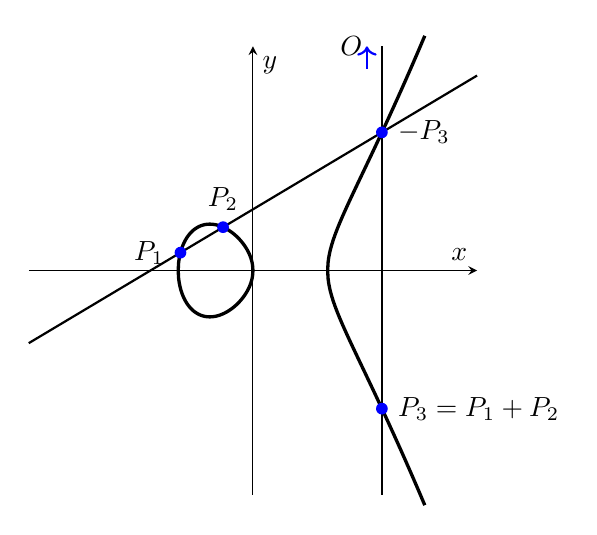
\begin{tikzpicture}[
	% define the style `point' which is used for the nodes on the coordinates
	point/.style={
		circle,
		fill=blue,
		inner sep=1.5pt,
	},
	]
	\begin{axis}[
	xmin=-3,
	xmax=3,
	ymin=-3,
	ymax=3,
	xlabel={$x$},
	ylabel={$y$},
	xtick={0},
	ytick={0},
%	scale only axis,
	axis lines=middle,
	% set the minimum value to the minimum x value
	% which in this case is $-\sqrt[3]{7}$
	samples=200,
	smooth,
	% to avoid that the "plot node" is clipped (partially)
	clip=false,
	% use same unit vectors on the axis
	axis equal image=true,
	]
	\addplot [black,very thick,domain=-1:0] {sqrt(x^3-x)};
	\addplot [black,very thick,domain=-1:0] {-sqrt(x^3-x)};
	\addplot [black,very thick,domain=1:2.3] {sqrt(x^3-x)};
	\addplot [black,very thick,domain=1:2.3] {-sqrt(x^3-x)};
	\addplot [black,thick,domain=-3:3] {0.596885079*x+0.818409101678};	
	\draw[thick] (1.726,-3) -| (1.726,3);
	\draw[blue,->,thick] (1.526,2.7) -| (1.526,3);
	% add nodes to the points and the corresponding labels
	\node [point,label={left:$P_1$}]
	(P1) at (-0.97,0.239)  {};
	\node [point,label={above:$P_2$}]
	(P2) at (-0.4,0.58)  {};
	\node [point,label={right:$-P_3$}]
	(P3) at (1.726,1.849)  {};
	\node [point,label={right:$P_3 = P_1 + P_2$}]
	(R)  at (1.726,-1.849) {};
	\node [label={left:$O$}]
	(O)  at (1.726,3) {};
	\end{axis}
	\end{tikzpicture}
	$$y^2=(x-\alpha_1)(x-\alpha_2)(x-\alpha_3)$$
	\caption{}
	\label{fig1}
\end{minipage}
\end{figure}
对椭圆曲线$\mathcal{C}:y^2=ax^3+bx^2+cx+d$,在仿射坐标卡$\mathcal{U}_2:=\left\{[x:y:1] \in \mathbb{CP}^2\right\} \cong \mathbb{C}^2$下, $\mathcal{C} \cap \mathcal{U}_2=\mathcal{C} \smallsetminus \{O\}$,我们可以显式地表示这个加法运算:
\begin{itemize}
	\item 当 $x_1 \neq x_2$, $$(x_1,y_1)+(x_2,y_2)=\left(x_3:=\lambda^2-a-x_1-x_2, \lambda (x_3-x_1)+y_1 \right), \text{ 其中 } \,\lambda=\frac{y_2-y_1}{x_2-x_1};$$
	\item  当$x_1 = x_2, y_1 \neq y_2$, $(x_1,y_1)+(x_2,y_2)=O$;
	\item 当$(x_1,y_1)=(x_2,y_2)=(x_0,y_0)$,
	\begin{equation}\label{eq:double}
		2(x_0,y_0)=\left(\frac{1}{4a}\frac{a^2x_0^4-2acx_0^2-8adx_0+c^2-4bd}{ax_0^3+bx_0^2+cx_0+d} \;\raisebox{-5pt}{,}\quad\frac{\phantom{66}}{\phantom{66}}\quad\right)
	\end{equation}
	方程(\ref{eq:double})被称为“双倍公式”;
	\item $O+(x_0,y_0)=(x_0,y_0)+O=(x_0,y_0); \qquad O+O=O$.
\end{itemize}
\begin{remarks}\
	\begin{itemize}
		\item 可以看出,这些显式运算均只用到了四则运算,故由封闭性,有理/实椭圆曲线可以视作复椭圆曲线的子群,亦为Abel群.
		\item 事实上,我们同样可以使用上述公式来给出并验证一般域$K$(e.g. $\;\mathbb{F}_p,\mathbb{Q}_p$)上椭圆曲线上的群结构.但是在实践中往往发现:
		\begin{itemize}
			\item 这样的定义较为丑陋,且过于依赖坐标卡;
			\item 须进行繁琐的分类讨论,特别是验证结合律时,且计算较复杂.事实上,椭圆曲线上的($K$-)点和$\deg 0$的可逆层(在层同构的意义下)一一对应,而可逆层关于张量积构成一个群.可以参考\cite[Proposition 19.9.3]{vakil2017rising}.
		\end{itemize}
		\item 椭圆曲线上的整点\footnote{严格来说,是$E\smallsetminus \{O\}$上的整点.}一般不为Abel群!事实上,由Siegel定理(1928),在仿射坐标卡上, $E$上只有有限多整点;另外,由Nagell-Lutz定理(1935,1937)(陈述与证明见\cite[p56, Theorem 2.5]{silverman1992rational}), $\mathbb{Q}$上椭圆曲线的挠点一定为整点.这两个定理较为精准地描绘出整点在椭圆曲线理论中的地位.
	\end{itemize}
\end{remarks}

我们现在陈述这篇小论文的中心定理:
\begin{theorem}[Mordell定理]
	设$K$为数域,则椭圆曲线$$E/K:y^2=4x^3+g_2x+g_3 \qquad g_2,g_3 \in K$$
	上的$K$-点关于上述群运算构成\CJKunderdot{有限生成}Abel群.
\end{theorem}
假设这个定理成立,那么由有限生成Abel群结构定理,我们有直和分解:
$$E(K) \cong \mathbb{Z}^{r} \times E(K)_{\tor}$$
我们称$r$为椭圆曲线$E(K)$的\textbf{秩(rank)}, $E(K)_{\tor}$为$E(K)$的\textbf{挠部分(Torsion Part)}.
\begin{remark}
	下面这些刻画椭圆曲线的结论已是人尽皆知,虽然证明它们尚费功夫.
	\begin{itemize}
		\item 对挠部分的刻画:
		\begin{itemize}
			\item 由Nagell-Lutz定理,椭圆曲线$E(K)$上的挠点一定为整点,且坐标有界(这意味着挠部分理论上一定是可以算出的)
			\item 由Mazur定理(1977),当$K=\mathbb{Q}$时, $E(K)_{\tor}$同构于循环群$\mathbb{Z}/N\mathbb{Z}\,(1 \leqslant N \leqslant 12,\, N \neq 11)$或$\mathbb{Z}/2\mathbb{Z} \times \mathbb{Z}/(2N\mathbb{Z}) \,(1 \leqslant N \leqslant 4)$,并且这几种情况都可能发生.
			\item []对给定数域$K$, 椭圆曲线的挠部分也只有有限种情况(Lo\"{i}c Merel于1996年证明,用到模曲线的理论).
			\item []而对Abel簇(\textbf{Torsion 猜想}:对于数域$K$上维数为$n$的Abel簇,挠部分只有有限种情况),至今仍是一个未解之谜.
		\end{itemize}
	\item 对无挠部分的刻画:
	\begin{itemize}
		\item 这是较难的部分,至今人类尚无找到一个切实有效的计算方法.BSD猜想给出了其与解析理论的联系,我们将在后文陈述.
		\item 类似地,类比Mazur定理,人们同样希望对椭圆曲线秩的可能性做出刻画.但是,构造高秩的椭圆曲线异常困难.(目前有人造出了秩大于27的椭圆曲线,但却不知道其具体的rank).尽管如此,我们还是有如下猜想:
		\begin{conj}
			椭圆曲线 $E/\mathbb{Q}$的rank可以达到任意大.
		\end{conj}
	\end{itemize}
	\end{itemize}
\end{remark}
\begin{remark}
	对亏格大于1、几何不可约的1维光滑$K$-射影簇, Faltings定理(1983, Faltings)告诉我们其上的有理点必为有限集.(同样是类似的“有限性”,证明中也同样用到了高的性质)这种随亏格变化而变化的性质与黎曼面的自同构群有些类似.
\end{remark}
\begin{eg}
	对椭圆曲线 $\mathcal{C}:y^2=x^3-x$的有理解只有$A:(0,0),B:(1,0),C:(-1,0)$,故该曲线满足Mordell定理.

		对$\frac{m}{n} \in \mathbb{Q}$, $m,n$互质,定义有理数的高
		$$H(\frac{m}{n}) = \max (|n|,|m|)$$
		定义椭圆曲线上有理点的高
		$$H(X)=H(x(X)) \qquad H(O)=1$$
		另外,为了符号简便,记$\mathcal{C}'=\mathcal{C} \smallsetminus \{A,B,C,O\}$.
		\begin{lemma}
			若$X=(x_0,y_0) \in \mathcal{C}'$, $x_0=\frac{m}{n}$, $m,n$互质,则
			\begin{enumerate}
				\item $H(-X)=H(X)$\label{lemma:en1}
				\item $H(X+A)=H(X)$\label{lemma:en2}
				\item 若$m,n$为奇数,则$H(X+B)<H(X)$\label{item:X+B}\label{lemma:en3}
				\item $H(2X)>H(X)$\label{lemma:en4}
			\end{enumerate}
		\end{lemma}
		\begin{proof}[引理的证明]
			经过计算可以得到.例如,
			\begin{enumerate} 
				\item[\textit{(3)}]
				\begin{equation*}
				\begin{aligned}
				\\[-1.3cm]
				H(X+B)=&H\left(\frac{x_0+1}{x_0-1}\right)=H\left(\frac{\frac{1}{2}(m+n)}{\frac{1}{2}(m-n)}\right)\\
				\leqslant&\max\left\{\frac{|m+n|}{2},\frac{|m-n|}{2}\right\}\\
				<&\max\left\{|m|,|n|\right\}
				\end{aligned}
				\end{equation*} 
				\item[\textit{(4)}] 
				\begin{equation*}
				\begin{aligned}[d]
				\\[-1.2cm]
				H(2X)=&H\left(\frac{(x_0^2+1)^2}{4(x_0^3-x_0)}\right)=H\left(\frac{(m^2+n^2)^2}{4mn(m^2-n^2)}\right)\\
				&\hspace{-5cm}\text{考察分子分母公因子,至多为4,}\\
			\leqslant&\max\left\{\frac{|m+n|}{2},\frac{|m-n|}{2}\right\}\\
				<&\max\left\{|m|,|n|\right\}=H(X)
				\end{aligned}
				\end{equation*}
			\end{enumerate}			
		\end{proof}
	\begin{proof}[例 3.6的证明]
		只需证$\mathcal{C}'=\varnothing$.我们使用反证法,若$\mathcal{C}'\neq\varnothing$,则取$X=(x_0,y_0) \in \mathcal{C}'$使得$H(X)$最小,并设$x_0=m/n$, $m,n$互质.
				
		不妨设$x(X)>1$(否则由\textit{(\ref{lemma:en2})},考虑$X+A$);
		由
		$$y_0^2=(x_0-1)x_0(x_0+1)=\frac{mn(m-n)(m+n)}{n^4}$$
		当$m,n$均为奇数时,由\textit{(\ref{lemma:en3})}, $H(X+B)<H(X)$,与$H(X)$最小性矛盾!故此时$m,n$一偶一奇, $m,n,m-n,m+n$两两互素,故均为有理数(整数)的平方,我们得到$x_0-1,x_0,x_0+1$均为有理数平方,设为$u^2,v^2,w^2$;
		
		我们取$Y=(v^2+uv+vw+wu,(u+v)(v+w)(w+u))$,可验证
		$$Y \in \mathcal{C}', \qquad X=2Y$$
		此时由\textit{(\ref{lemma:en4})}, $H(Y)<H(X)$,与$H(X)$最小性矛盾!
	\end{proof}
\begin{remark}
	这个证明显示了椭圆曲线上高的威力.通过与椭圆曲线上群运算相联系,我们构造出高更小的点,从而导出矛盾.之后在一般的椭圆曲线上,我们还会建立类似的与高相关的不等式.
	
	另外,使用类似的方法,可以说明$y^2=x^3-N^2x$, $N=1,2,3$均无$y\neq0$的有理解,这说明$1,2,3$均不为某个边长为有理数的直角三角形的面积.
\end{remark}
\end{eg}
\clearpage
\section{简要思路与无穷递降法}
Mordell定理的证明,在大部分书中(如\cite{fermat2013dream}\cite{tate1974the}),为了逻辑思路的清晰,一律使用执果索因的方法,其证明的整体框架如下:
\begin{figure}[th]
	\begin{minipage}[t]{\textwidth}
		\centering
\tikzstyle{startstop} = [rectangle, minimum width=3cm,minimum height=1cm,text centered, draw=black,fill=red!30]

\tikzstyle{part} = [rectangle,minimum width=6cm,minimum height=10cm,left,text width =6cm,draw=black,fill=yellow!30]
\tikzstyle{prop} = [rectangle,minimum width=5cm,minimum height=1cm,left,text width =5cm]
\tikzstyle{arrow} = [thick,->,>=stealth]
\tikzstyle{arrow2} = [thick,<->,>=stealth]
\begin{tikzpicture}[node distance=3cm]
\node (start) [startstop] {Mordell定理};
\node (part1) [part,below of=start,yshift=-6cm,xshift=-4cm]{};
\node (part2) [part,right of=part1,xshift=5cm] {};
\draw [<-,shorten <=3pt,semithick] (start) -- node[right]{无穷递降法}(0,-3);
\draw [semithick] (-6.5,-12) |- (4,-3)-|(4,-6);
\node [above of=part1,text width=7cm,yshift=1.5cm,xshift=0.5cm]
{\colorbox{yellow!30}{高的性质} };
\node [above of=part2,text width=7cm,yshift=1.5cm,xshift=0.5cm]{\colorbox{yellow!30}{弱Mordell定理}};
\draw [semithick] (-6.5,-6.3) |- (-6.3,-6.3);\draw [semithick](-6.5,-8.3) |- (-6.3,-8.3);\draw [semithick](-6.5,-10.3) |- (-6.3,-10.3);
\node (prop1)[prop,above of=part1,yshift=-0.3cm,xshift=0.5cm]{$\#\{P \mid H(P)\!<\!M \}< + \infty$};
\node (prop2)[prop,below of=prop1,yshift=1cm]{$H(P+Q) \leqslant C_1H(P)^2$};
\node (prop3)[prop,below of=prop2,yshift=1cm]{$H(P)^4 \leqslant C_2H(2P)$};
\node (prop4)[prop,text centered,right of=prop1,xshift=4.5cm]{$\#E(K)/mE(K)< + \infty$};
\node (prop5)[prop,text centered,below of=prop4,yshift=1cm]{$[K\big([m]^{-1}E(K)\big):K]\!<\! + \infty$};
\node (prop6)[prop,text centered,below of=prop5,yshift=1cm]{$\#T_S\! <+\! \infty$};
\node (prop7)[prop,text centered,below of=prop6,yshift=1cm]{$R_S^{\times}\text{ 为有限生成群}$};
\draw [<-,shorten <=3pt,semithick] (prop4) to (prop5);
\draw [<-,shorten <=3pt,semithick] (prop5) to (prop6);
\draw [<-,shorten <=3pt,semithick] (prop6) to (prop7);
\end{tikzpicture}
	\caption{}
\label{fig2}
\end{minipage}
\end{figure}

从逻辑框图中可以看出, Mordell定理的证明主要包括两个部分:椭圆曲线上高的性质和商群的有限生成性.我们已经在上一节的例子中看到椭圆曲线的高在证明中起的关键作用.粗略来说,高体现了一个点的复杂程度,相当于给这些点按照重要程度分类;通过将最重要的点与$E(K)/mE(K)$(在$E(K)$上)的代表元合在一起,即可给出$E(K)$的生成元集,而这便是无穷递降法的思维方式.

在这一节中,我们假设弱Mordell定理的正确性,尝试对$K=\mathbb{Q}$的情况完成证明.

我们定义椭圆曲线$E/\mathbb{Q}:y^2=x^3+Ax+B$上的\textbf{Naive height}:
%$H:E(\mathbb{Q}) \longrightarrow \mathbb{N}^+$
设$P \in E(\mathbb{Q})$,
\begin{itemize}
	\item $P=O$.令$H(O)=1$;
	\item $P \neq O$.设$x(P)=m/n$, $m,n$互质,则
	$$H(P):=\max \{|m|,|n|\}$$
\end{itemize}
我们定义的Naive height有如下性质:
\begin{proposition}[Naive height]\label{prop:naiveht}\
	\begin{enumerate}[1.]
		\item (有限性)对任意$M>0$, $\#\{P \in E(\mathbb{Q})\mid H(P)<M \} < + \infty$
		\item (加法)设$Q \in E(\mathbb{Q})$,则存在$C_1=C_1(Q,E/\mathbb{Q})$使得
		$$H(P+Q) \leqslant C_1H(P)^2 \quad\text{ for any }P \in E(\mathbb{Q})$$
		\item (数乘)存在$C_2=C_2(E/\mathbb{Q})$使得
		$$H(P)^4 \leqslant C_2H(2P) \quad\text{ for any }P \in E(\mathbb{Q})$$
	\end{enumerate}
\end{proposition}
\begin{proof}\
	\begin{enumerate}[1.]
		\item 显然.
		\item 本质就是展开计算.设$$ P=(x,y)=\left(\frac{a}{d^2},\frac{b}{d^3}\right),\qquad P_0=(x_0,y_0)=\left(\frac{a_0}{d_0^2},\frac{b_0}{d_0^3}\right), $$其中$\gcd (a,b,d)=\gcd(a_0,b_0,c_0)=1$.
		则\begin{equation*}
		\begin{aligned}
		&b^2=a^3+Aad^4+Bd^6\\
		\Longrightarrow& \gcd(a,d)=1\\
		\Longrightarrow&H(P)=\max\{|a|,|d|^2\}
		\end{aligned}
		\end{equation*}
		\begin{equation*}
		\begin{aligned}
		x(P+P_0)=&\left(\frac{y-y_0}{x-x_0}\right)^2-x-x_0\\
		=& \frac{x^3+Ax+B-2yy_0+x_0^3+Ax_0+B-(x+x_0)(x-x_0)^2}{(x-x_0)^2}\\
		=&\frac{(x+x_0)(xx_0+A)+2B-2yy_0}{(x-x_0)^2}\\
		=&\frac{(a_0a+Ad_0^2d^2)(d_0^2a+a_0d^2)+2Bd_0^4d^4-2b_0d_0bd}{(d_0^2a-a_0d^2)^2}\\
		\leqslant&C_1' \max \{|a|^2,|d|^4,|bd|\}\\
		\leqslant& C_1 \max \{|a|^2,|d|^4\}=C_1H(P)^2
		\end{aligned}
		\end{equation*}
		其中
		\begin{equation*}
		\begin{aligned}
		|bd|^2=&|(a^3+Aad^4+Bd^6)d^2|\\
		\leqslant& C''^2 \max \{|a|^4,|d|^8\}\\
		=&(C'' \max \{|a|^2,|d|^4\})^2
		\end{aligned}
		\end{equation*}
		注意到我们的讨论遗漏了$P_0=O,P=O$与$P= \pm P_0$的特殊情况,只需适当调节$C_1$即可.(以$\max\{H(P_0),H(2P_0),C_1\}$代替$C_1$).
		\item 同样我们不考虑$P=O$及$2P=O$的情况.设$x(P)=m/n$, $m,n$互素,由双倍公式,
		\begin{equation*}
		\begin{aligned}
		x(2P)=&\frac{1}{4}\frac{x_0^4-2Ax_0^2-8Bx_0+A^2}{x_0^3+Ax_0+B}\\
		=&\frac{1}{4}\frac{m^4-2Am^2n^2-8Bmn^3+A^2n^4}{n(m^3+Amn^2+Bn^3)}
		\end{aligned}
		\end{equation*}	
		令
		$$\begin{cases}
			F(m,n)=m^4-2Am^2n^2-8Bmn^3+A^2n^4\\
			G(m,n)=4n(m^3+Amn^2+Bn^3)
		\end{cases}$$	
		我们希望刻画$F(m,n)$与$G(m,n)$的最大公因子.由于$$F(m,n)=\frac{1}{16n^2}\left(\frac{\partial G}{\partial m}(m,n)\right)^2-2\frac{m}{n}G(m,n)$$
		我们有$Z(F,G)=\{(0,0)\}$ in $\mathbb{A}_K^2$. (这可以在去齐次化之后清楚地看到,设$f(x)=F(x,1),g(x)=G(x,1)$,则有
		$$f(x)=\frac{1}{16}(g'(x))^2-2mg(x), $$
		而$g(x)$无重根,故$f(x),g(x)$互素,无公共根) 由Hilbert零点定理,
		$$\sqrt{(F,G)}=(x,y)$$
		故存在$\tilde{b}_1,\tilde{b}_2,\tilde{b}_3,\tilde{b}_4 \in \mathbb{Q}[x,y], r_1,r_2 \in \mathbb{N}^+$,使得
		$$\begin{cases}
		\tilde{b}_1F+\tilde{b}_2G=x^{r_1}\\
		\tilde{b}_3F+\tilde{b}_4G=y^{r_2}
		\end{cases}$$
		约去分母,取$r=\max \{r_1,r_2\}$配平后,存在$b_1,b_2,b_3,b_4 \in \mathbb{Q}[x,y], R,r \in \mathbb{N}^+$,使得\footnote{在\cite[p222, Sublemma 4.3]{tate1974the}中给了具体的$b_i,R,r$值的某一个可能.}
		\begin{equation}\label{eq:UFD}
			\begin{cases}
			b_1(x,y)F(x,y)+b_2(x,y)G(x,y)=Rx^r\\
			b_3(x,y)F(x,y)+b_4(x,y)G(x,y)=Ry^r
			\end{cases}
		\end{equation}		
		注意这里的$R$与$x,y$无关,只与$A,B$相关.另外可以通过去掉重复项来假设$b_1 \sim b_4$均为次数为$r-4$的齐次多项式.
		
		取$k \in \mathbb{N}^+$,使$kA^2,kB \in \mathbb{Z}$,则
		$$kF(x,y),kG(x,y) \in \mathbb{Z}[x,y]$$
		令$d=\gcd \{kF(x,y),kG(x,y)\}$,则
		$$\begin{cases}
		d\,|\,kRx^r\\
		d\,|\,kRy^r
		\end{cases} \Rightarrow d\,|\,kR$$
		故
		\begin{equation*}
		\begin{aligned}
		H(2P)=&H\left(\frac{F(m,n)}{G(m,n)}\right)\\
		=&H\left(\frac{kF(m,n)}{d} \middle/\frac{kG(m,n)}{d} \right)\\
		\geqslant &\frac{1}{R} \max \{|F(m,n)|,|G(m,n)|\}
		\end{aligned}
		\end{equation*}
		此时我们需要一个与$F,G$相关的估计.由方程(\ref{eq:UFD}),
		\begin{equation*}
		\begin{aligned}
			& \begin{cases}
			R|m|^r \leqslant 2\max \left\{|b_1(m,n)|,|b_2(m,n)|\right\}\max  \left\{|F(m,n)|,|G(m,n)|\right\}\\
			R|n|^r \leqslant 2\max \left\{|b_1(m,n)|,|b_2(m,n)|\right\}\max  \left\{|F(m,n)|,|G(m,n)|\right\}
			\end{cases}\\
			\Longrightarrow& 
			R\max\left\{|m|,|n|\right\}^r \leqslant \max \left\{|b_1(m,n)|,|b_2(m,n)|\right\}\max  \left\{|F(m,n)|,|G(m,n)|\right\}\\
			\phantom{\Longrightarrow}&\phantom{R\max\left\{|m|,|n|\right\}^r} \leqslant C_2\max \left\{|m|,|n|\right\}^{r-4}\max  \left\{|F(m,n)|,|G(m,n)|\right\}\\
			\Longrightarrow& H(2P)\geqslant \frac{1}{R} \max \{|F(m,n)|,|G(m,n)|\}\\
			\phantom{\Longrightarrow}&\phantom{H(2P)}\geqslant \frac{1}{C_2} \left\{|m|,|n|\right\}^{4}=\frac{1}{C_2}H^4(P)
		\end{aligned}
		\end{equation*}
	\end{enumerate}
\end{proof}

有了这些性质,再假设$E(\mathbb{Q})/2E(\mathbb{Q})$为有限群(弱Mordell定理成立),我们便可以轻而易举地使用“无穷递降法”得到所需的性质.
\begin{theorem}[无穷递降法]
	设椭圆曲线 $E(\mathbb{Q})$满足\textbf{命题 \ref{prop:naiveht}},且$E(\mathbb{Q})/2E(\mathbb{Q})$为有限群,则$E(\mathbb{Q})$为有限生成Abel群.
\end{theorem}
\begin{proof}
	为了方便处理,我们令$h(P)=\log H(P)$, 重新叙述\textbf{命题 \ref{prop:naiveht}}:
	\begin{proposition}\label{prop:naiveht2}\
		\begin{enumerate}
			\item 对任意$M>0$, $\#\{P \in E(\mathbb{Q})\mid h(P)<M \} < + \infty$
			\item 设$Q \in E(\mathbb{Q})$,则存在$C_1=C_1(Q,E/\mathbb{Q})>0$使得
			$$h(P+Q) \leqslant C_1(Q)+2h(P)\quad\text{ for any }P \in E(\mathbb{Q})$$
			\item 存在$C_2=C_2(E/\mathbb{Q})>0$使得
			$$4h(P) \leqslant C_2+h(2P) \quad\text{ for any }P \in E(\mathbb{Q})$$
		\end{enumerate}
	\end{proposition}
设$E(\mathbb{Q})/2E(\mathbb{Q})$的代表元为$Q_1, \ldots , Q_k$,取$C_0=\sum_{i=1}^{k}C_1(Q_i)+C_2$,则
$$\Sigma:=\{P \in E(\mathbb{Q})\mid h(P)<C_0 \} \cup \{Q_i\}_{i=1}^k$$
是一个有限集.下证明$\Sigma$为$E(\mathbb{Q})$的生成元集:

若否,取不被生成的点中高最小的点$P_0 \in E(\mathbb{Q})$,故存在$j, R \in E(\mathbb{Q})$使得
$$P_0-Q_j=2R$$
$R$必不能被$\Sigma$有限生成,故$h(P_0)\leqslant h(R)$.另外,我们有
\begin{equation*}
\begin{aligned}
h(R) \leqslant & \frac{1}{4}(C_2+h(P_0-Q_j))\\
\leqslant & \frac{1}{4}(C_2+C_1(Q_j)+2h(P))\\
\leqslant & \frac{1}{4}(C_0+2h(P))\\
\leqslant & \frac{1}{4}(C_0+2h(R))\\
\end{aligned}
\end{equation*}
得到$h(R) \leqslant C_0/2$, $R \in \Sigma$,矛盾!
\end{proof}


\section{弱Mordell定理的证明}
在这一节中,我们将按照从特殊到一般的方式,给出弱Mordell定理不同版本的证明:
\begin{itemize}
	\item 在引理 \ref{eg:weakMT}中,处理$\mathbb{Q}$上特殊的椭圆曲线处理弱Mordell定理($m=2$);
	\item 利用初等的代数方法证明弱Mordell定理($m=2$);
	\item 使用对域扩张的有限性刻画,应用分歧理论证明弱Mordell定理;
	\item 利用Selmer群的有限性证明弱Mordell定理.
\end{itemize}
笔者最喜欢首尾两个证明,前者将问题简化至初等数论的范围内即可解决的问题,而后者引出了椭圆曲线上极为重要的量并深刻刻画了它们之间的关系,而且可以较易推广至一般的Abel簇上.读者宜自行取舍,事实上,第二个证明即已足够给出一般数域上Mordell定理的完整证明.
\begin{eg}\label{eg:weakMT}
	在教材\cite{fermat2013dream}中提到了对$\mathbb{Q}$上形如
	\begin{equation}\label{eq:ellsplit}
	y^2=(x-a)(x-b)(x-c)
	\end{equation}
	的椭圆曲线,通过$x$坐标给出的椭圆曲线至$\mathbb{Q}^{\times}/(\mathbb{Q}^{\times})^2$的群同态,证明了弱Mordell定理($m=2$).注意在该证明过程中用到了$\mathbb{Q}$的代数整数环$\mathbb{Z}$是UFD的性质.
\end{eg}
\subsection{Galois上同调的引入(工具)}\phantom{1}

不失一般化,设$L$为$K$的代数扩张(e.g.$\;L=\bar{K}$), $G=\Gal(L/K)$.为了描述函子$(\cdot)^G: \Mod_{\mathbb{Z}[G]} \longrightarrow \Grp$,我们引入Galois上同调,注意这是有限群上同调的推广.

给定群$G$以投射有限(profinite)拓扑, Abel 群$M$以离散拓扑,设$G$在$M$上连续作用,也就是
$$ \text{For any } m \in M,\qquad [\Gal(\bar{K}/K):\Stab(m)] < +\infty$$
我们定义链复形
$$C^0(G,M):=M\qquad C^k(G,M):= \left\{\xi: G^k \rightarrow M \mid \xi \text{连续}\right\} \text{ for } k\geqslant 1$$
以及微分运算
$$d_k:C^k(G,M) \longrightarrow C^{k+1}(G,M)$$
\begin{equation*}
\begin{aligned}
d_k\xi (\sigma_1, \ldots,\sigma_{k+1})=&\phantom{+}\sigma_1\xi (\sigma_2, \ldots , \sigma_{k+1})\\
&+\sum_{i=1}^{k}(-1)^i\xi (\sigma_1, \ldots,\sigma_i\sigma_{i+1}, \ldots,\sigma_{k+1})\\
&+(-1)^{k+1}\xi (\sigma_1,\ldots,\sigma_k)
\end{aligned}
\end{equation*}
可以验证$d^2=0$,我们得到上同调群$$H^k(G,M):=\Ker d_k /\Img d_{k-1}$$
(当$k<0$时, $C^k(G,M):=0, \quad d_k:=0.$)
还可以验证:
\begin{itemize}
	\item $(d_0 m) (\sigma)=\sigma(m) -m, 	\qquad (d_1 \xi) (\sigma_1,\sigma_2)=\sigma_1 \xi(\sigma_2)-\xi(\sigma_1\sigma_2)+\xi(\sigma_1);$
	\item \phantom{1}\\[-1cm] $$H^0(G,M)=\left\{m \in M \mid \sigma(m)=m\right\}=M^G;$$
	$$H^1(G,M)=\frac{\displaystyle\left\{\xi \in C^1(G,M) \mid \xi (\sigma_1\sigma_2)=\sigma_1(\xi(\sigma_2))+\xi(\sigma_1)\right\}}{\displaystyle\left\{\xi \in C^1(G,M) \mid\exists\, m \in M,\forall\,\sigma \in G, \xi(\sigma)=\sigma(m)-m\right\}}\;\raisebox{-10pt}{;}$$
	\item 对$G$-模正合列($G$的作用均连续)
	$$0 \longrightarrow P \longrightarrow M \longrightarrow N \longrightarrow 0$$
	我们有长正合列
	\begin{center}
		\begin{tikzcd}
			& {H^1(G,P)} \arrow[r] & {H^1(G,M)} \arrow[r]\arrow[d, phantom, ""{coordinate, name=Z}] & {H^1(G,N)} \\
			0 \arrow[r] & P^G \arrow[r]        & M^G \arrow[r]        & N^G  \arrow[ull,
			"\delta"',
			rounded corners = 11,
			to path={ -- ([xshift=5ex]\tikztostart.east)
				|- (Z) [near end]\tikztonodes
				-| ([xshift=-5ex]\tikztotarget.west)
				-- (\tikztotarget)}]     
		\end{tikzcd}	
	\end{center}
\end{itemize}
(事实上我们最关心的是这个长正合列而不是微分$d_k$的方式)
\begin{remark}
	在某些文献中,记$WC(E/K):= H^1(\Gal (\bar{K}/K),E(\bar{K}))$,称其为椭圆曲线$E/K$的\textbf{Weil-Ch\^{a}telet群}.
	
	事实上,当$G$为有限群时, $H^n(G,M)=\Ext^n_{\mathbb{Z}[G]}(\mathbb{Z},M)$, Galois上同调就是函子$(\cdot)^G=\Hom(\mathbb{Z},-)$的导出函子.
\end{remark}
\begin{theorem}[弱Mordell定理]
	设$K$为数域, $E/K$为椭圆曲线, $m \in \mathbb{N}^+$, 则$E(K)/mE(K)$为有限群.
\end{theorem}
对一般的椭圆曲线
$$y^2=ax^3+bx^2+cx+d, $$
我们同样希望写成(\ref{eq:ellsplit})的形式,但方程$ax^3+bx^2+cx+d=0$根可能跳出$\mathbb{Q}$的范围.下面这个引理说明,我们可以用添根的办法,尝试在更大的域中处理弱Mordell定理.
\begin{lemma}[有限域扩张与弱Mordell定理的关系]
	设$L/K$为有限Galois扩张,则
	$$\#E(L)/mE(L) < + \infty \quad \Longrightarrow \quad \#E(K)/mE(K) < + \infty$$
\end{lemma}
\begin{proof}
	我们有正合列
	\begin{center}
		\begin{tikzcd}
			0 \ar{r}   & 
			\Ker \phi \ar{r}\ar[equal]{d}& 
			E(K)/mE(K) \ar{r}{\phi}&
			E(L)/mE(L) \\
			& \displaystyle\frac{\displaystyle E(K)\cap mE(L)}{\displaystyle mE(K)}&&\\
		\end{tikzcd}
	\end{center}

只需证$\#\Ker \phi < + \infty$即可.令$G=\Gal(L/K)$,对正合列
	\begin{center}
	\begin{tikzcd}
		0 \arrow[r] & {E(L)[m]} \arrow[r] & E(L) \arrow[r, "m(-)"] & mE(L) \arrow[r] & 0
	\end{tikzcd}
	\end{center}
作用函子$(\cdot)^G$,诱导长正合列
	\begin{center}
	\begin{tikzcd}
		0 \arrow[r] & {E(K)[m]} \arrow[r]     & E(K) \arrow[r, "m(-)"]    & E(K) \cap mE(L)\arrow[r]   & {H^1(G,E(L)[m])}            
	\end{tikzcd}
	\end{center}
得到单射
$$\Ker \phi=\frac{E(K) \cap mE(L)}{mE(K)} \hookrightarrow H^1(G,E(L)[m])$$
故$\#\Ker \phi < + \infty$.
\iffalse%%%%%%%%%%%%%%%%%%%%%%%%%%%%%%%%%%%%%%%%%%注释
对每一个$\bar{P} \in \Ker \phi$(后省略代表元符号),设$P=nQ$, $Q \in E(L)$,我们指定一个良定映射(与$Q$相关)
$$\lambda_P: \Gal (L/K) \longrightarrow E(L)[m] \qquad \sigma \longmapsto \sigma(Q)-Q$$
于是我们得到一个非自然的映射:
$$\Phi \longrightarrow \Hom_{\Set}(\Gal (L/K), E(L)[m]) \qquad P \longmapsto \lambda_P$$
可以验证$\Phi$为单射:
\begin{equation*}
\begin{aligned}
\Phi(P)=\Phi(P') \Longrightarrow&\; \sigma(Q)-Q=\sigma(Q')-Q' \quad\text{ for any } \sigma \in \Gal(L/K)\\
\Longrightarrow&\;\sigma(Q-Q')=Q-Q'\quad\text{ for any } \sigma \in \Gal(L/K)\\
\Longrightarrow&\;Q-Q' \in E(K)\\
\Longrightarrow&\;P-P'=m(Q-Q')=0 \quad{ in } \;\Ker \phi\\
\end{aligned}
\end{equation*}
故$\#\Ker \phi < + \infty$.
\fi%%%%%%%%%%%%%%%%%%%%%%%%%%%%%%%%%%%%%%%%%%注释
\end{proof}

\begin{remark}\
	在这之后,我们可以假设
	\begin{itemize}
		\item 椭圆曲线的形式为$y^2=(x-a)(x-b)(x-c),\quad a,b,c \in K$;
		\item $E[m]:=E(\bar{K})[m]\subseteq E(K)$
		\item 椭圆曲线的形式为$y^2=(x-a)(x-b)(x-c),\quad a,b,c \in \mathcal{O}_K$;\\
		(取$t \in K$使得$t^2a,t^2b,t^2c \in \mathcal{O}_K$,则$(t^3y)^2=(t^2x-t^2a)(t^2x-t^2b)(t^2x-t^2c)$.)
		\item $K$包含$n$次单位根$\mu_m$;
		\item 我们甚至可以假设$a+b+c=0$.当然这个假设在下文中没有起到作用.
	\end{itemize}
\textbf{在接下来的第五小节中,为方便起见,我们均作如上假设.}
%当$E[m] \subseteq E(K)$时,我们给出的映射$\lambda_P$与$Q$无关, $\Phi$ 也是自然的映射,注意到这里$E(K)=E(L)^{\Gal(L/K)}$.

\end{remark}
\subsection{m=2的情况}\phantom{1}

但我们想追随\textit{例} \ref{eg:weakMT}时发现这个证明并不能照搬无误地推广,因为代数整数环一般不是UFD.不过,根据\textbf{定理 \ref{thm:idealclass}},代数整数环“离UFD只有有限的距离”,这给了迷茫的我们一点希望.同样设椭圆曲线$E/K:y^2=(x-e_1)(x-e_2)(x-e_3), e_1,e_2,e_3 \in \mathcal{O}_K$.
\subsection*{\underline{Step1}}我们定义映射(补充定义$e_4=e_1,e_0=e_3$)($i \in \{1,2,3\}$)
\begin{equation*}
\begin{aligned}
\tilde{\varphi}_i:E(K) &\longrightarrow K^{\times}\\
\hspace{3mm}O\hspace{3mm}& \longmapsto 1\\
(e_i,0)&\longmapsto (e_{i+1}-e_i)(e_{i-1}-e_i)\\
(x,y) &\longmapsto x-e_i \hspace{2cm}\text{ 若 }y \neq 0
\end{aligned}
\end{equation*}
	\begin{center}
	\begin{tikzcd}
		\varphi_i:=\pi \circ \tilde{\varphi}_i:E(K)  \arrow[r, "\tilde{\varphi}_i"] & K^{\times} \arrow[r, "\pi"]     & K^{\times}/(K^{\times})^2     
	\end{tikzcd}
\end{center}
(某种意义上说,即是考虑椭圆曲线上点的横坐标)

我们验证$\varphi_i$为群同态,这等价于验证
\begin{center}
\fbox{\begin{minipage}{14cm}\phantom{1}\\[-0.2cm]
		\phantom{占位}对任意$P_1,P_2,P_3 \in E(K)$满足$P_1+P_2+P_3=O$,有
		\begin{equation}\label{eq:inKtimes}
		\varphi_i(P_1)\varphi_i(P_2)\varphi_i(P_3)=1 \qquad \text{ in }K^{\times}/(K^{\times})^2     
		\end{equation}\\[-1cm]
	\end{minipage}
}
\end{center}
对于特殊情况,即$P_1,P_2,P_3$中有元素为$O$或$(e_j,0)$时,易验证(\ref{eq:inKtimes})成立.当$P_1,P_2,P_3$均不为$O$或$(e_j,0)$时,记$x_j:=x(P_j)$,则欲证式成为
$$(x_1-e_i)(x_2-e_i)(x_3-e_i) \in (K^{\times})^2$$
由$P_1+P_2+P_3=O$知$P_1,P_2,P_3$三点共线,记该直线为$y=kx+b,\;k,b \in K$,连立方程(解为$P_1,P_2,P_3$)
\begin{equation*}
\begin{aligned}
&\begin{cases}
y=kx+b\\
y^2=(x-e_1)(x-e_2)(x-e_3)
\end{cases}\\
\Longrightarrow&(x-e_1)(x-e_2)(x-e_3)-(kx+b)^2=0 \qquad\text{ 有解 }x_1,x_2,x_3\\
\Longrightarrow&(x-e_1)(x-e_2)(x-e_3)-(kx+b)^2=(x-x_1)(x-x_2)(x-x_3)\\
\Longrightarrow&-(ke_i+b)^2=(e_i-x_1)(e_i-x_2)(e_i-x_3)\\
\Longrightarrow&(x_1-e_i)(x_2-e_i)(x_3-e_i)=(ke_i+b)^2 \in (K^{\times})^2\\
\end{aligned}
\end{equation*}
\subsection*{\underline{Step2}}
令
$$\varphi:E(K) \longrightarrow (K^{\times}/(K^{\times})^2)^3 \qquad P \longmapsto (\varphi_1(P),\varphi_2(P),\varphi_3(P))$$
则$\Ker \varphi =2E(K)$,故有$E(K)/2E(K) \cong \Img \varphi$.

首先由于群$(K^{\times}/(K^{\times})^2)^3$为2-Torsion群, $2E(K) \subseteq \Ker \varphi$.我们将证明$\Ker \varphi \subseteq 2E(K)$:设$P \in \Ker \varphi$,则
\begin{enumerate}[(i)]
	\item $P=O:\qquad O=2(e_1,0) \in 2E(K)$.
	\item $P=(e_1,0):$($P=(e_2,0)$或$(e_3,0)$同理)由$P \in \Ker \varphi$, $\;e_1-e_2,e_1-e_3$均为$K^{\times}$中数的平方,记为$v,w$,则
	$$e_1=v^2+e_2=w^+e_3$$
	令$Q=(e_1+vw,vw(v+w))$,可验证$Q \in E(K), P=2Q$.
	\item $y(P) \neq 0$,记$x_0:=x(P)$,则$x_0-e_1,x_0-e_2,x_0-e_3$均为$K^{\times}$中数的平方,记为$u,v,w$,故有
	$$u^2+e_1=v^2+e_2=w^2+e_3$$
	令$Q=(x_0+vw+wu+uv,(v+w)(w+u)(u+v))$,可验证$Q \in E(K), P=2Q$.
\end{enumerate}
\subsection*{\underline{Step3}}
为了除去$K$的单位元的影响,定义映射
$$\eta:K^{\times}/(K^{\times})^2 \longrightarrow P_K/(P_K)^2 \qquad \bar{x} \longmapsto [x]_{(P_K)^2}$$
则$\eta$为良定义的群同态,可以计算
\begin{equation*}
\begin{aligned}
\Ker \eta =& \left\{\bar{x} \in K^{\times}/(K^{\times})^2 \middle|\text{ 存在 }y \in K, u \in \mathcal{O}_K^\times, \text{ 使得 }x=uy^2 \right\}\\
=&\frac{\mathcal{O}_K^\times(K^{\times})^2}{(K^{\times})^2} \cong \frac{\mathcal{O}_K^\times \cap
	(K^{\times})^2}{\mathcal{O}_K^\times}=\frac{\mathcal{O}_K^\times}{(\mathcal{O}_K^\times)^2}
\end{aligned}
\end{equation*}
由\textbf{定理 \ref{thm:idealclass}}, $\mathcal{O}_K^\times$为有限生成Abel群,故$\# \Ker \eta < + \infty$.令
	\begin{center}
	\begin{tikzcd}[row sep = 0cm]
		\hat{\varphi}:E(K) \arrow[r, "\varphi"] &[-0.3cm] (K^{\times}/(K^{\times})^2)^3 \arrow[r, "{\hat{\eta}=(\eta,\eta,\eta)}"] & (P_K/(P_K)^2)^3 \\ P \arrow[rr, maps to] && {(\eta(\varphi_1(P)),\eta(\varphi_2(P)),\eta(\varphi_3(P)))}
	\end{tikzcd}
	\end{center}
由于$\Img \hat{\varphi} \cong \Img \varphi/(\Ker \hat{\eta} \cap \Img \varphi)$,而$\Img \varphi \cong E(K)/2E(K)$,只需证$\Img \hat{\varphi}$有限即可得到$m=2$时弱Mordell定理的结论.

在这一步中,我们通过将理想替代数,从而约去了有限生成Abel群$\mathcal{O}_K^\times$对像的影响.或者说,我们通过考虑单位群$\mathcal{O}_K^\times$在$(K^{\times}/(K^{\times})^2)^3$上作用的轨道来减少我们需要分析的元素个数.
\subsection*{\underline{Step4}}
我们将$\mathcal{O}_K$类比$\mathbb{Z}$,以理想类比数,得到一个对点$(x,y)$的刻画.这里毕竟不是UFD,故类群也将在此出没,将理想的性质转回数的性质.在 \textbf{\underline{Step4}}与 \textbf{\underline{Step5}}中,取定有限群$Cl(K)$的代表元$\mathfrak{m}_1,\ldots , \mathfrak{m}_n$(为方便起见,这里取$\mathcal{O}_K$的理想).记$(x):=x \mathcal{O}_K$.
\begin{lemma}\label{lem:value2&3ideal}
	对$(x,y) \in E(K), \;x,y\neq 0$,存在$\mathfrak{r},\mathfrak{s},\mathfrak{t} \vartriangleleft \mathcal{O}_K$,使得
	$$(x)=\frac{\mathfrak{r}}{\mathfrak{t}^2}, \qquad (y)=\frac{\mathfrak{s}}{\mathfrak{t}^3}, $$
	$$\gcd(\mathfrak{r},\mathfrak{t}^2)=\gcd (\mathfrak{s},\mathfrak{t}^3)=\mathcal{O}_K.$$
	这里$\gcd(\mathfrak{a},\mathfrak{b}):=\mathfrak{a}+\mathfrak{b}$. 具体地,若
	$$\mathfrak{a}=\prod_{i=1}^{g}\mathfrak{p}_i^{e_i} \qquad \mathfrak{b}=\prod_{i=1}^{g}\mathfrak{p}_i^{e_i'}$$
	则$$\gcd(\mathfrak{a},\mathfrak{b}):=\prod_{i=1}^{g}\mathfrak{p}_i^{\min (e_i,e_i')}$$
\end{lemma}
\begin{proof}
	记$\alpha=-(e_1+e_2+e_3), \beta=e_1e_2+e_2e_3+e_3e_1, \gamma =-e_1e_2e_3$,则$\alpha,\beta,\gamma \in \mathcal{O}_K$,且
	$$y^2=(x-e_1)(x-e_2)(x-e_3)=x^3+\alpha x^2 +\beta x+ \gamma$$
	对$\mathfrak{p} \in \MaxSpec O_K$,我们将证明
	$$v_{\mathfrak{p}}(x)<0 \Longleftrightarrow v_{\mathfrak{p}}(x)<0 \Longleftrightarrow \;\exists \; l \in \mathbb{N}^+, v_{\mathfrak{p}}(x)=-2l, v_{\mathfrak{p}}(y)=-3l. $$	
	“$\Longleftarrow$”的方向均显然,故只需证
	$$v_{\mathfrak{p}}(x)<0 \Longrightarrow \;\exists \; l \in \mathbb{N}^+, v_{\mathfrak{p}}(x)=-2l, v_{\mathfrak{p}}(y)=-3l.$$
	记$v_{\mathfrak{p}}(x)=-k$, $k \in \mathbb{N}^+$.由于
	\begin{equation*}
	\begin{aligned}
	&\begin{cases}
	v_{\mathfrak{p}}(x^3)=-3k&\\
	v_{\mathfrak{p}}(\alpha x^2+\beta x+ c)&\geqslant \min \left\{v_{\mathfrak{p}}(\alpha x^2),v_{\mathfrak{p}}(\beta x),v_{\mathfrak{p}}(c)\right\}\\
	&\geqslant \min \left\{v_{\mathfrak{p}}(\alpha )-2k,v_{\mathfrak{p}}(\beta)-k,v_{\mathfrak{p}}(c)\right\}\\
	&\geqslant -2k>-3k
	\end{cases}\\
	\Longrightarrow & 2v_{\mathfrak{p}}(y)=v_{\mathfrak{p}}(x^3+(\alpha x^2+\beta x+ c))=-3k
	\end{aligned}
	\end{equation*}
	故$k$为偶数,记$k=2l$,则$v_{\mathfrak{p}}(x)=-2l,v_{\mathfrak{p}}(y)=-3l$.此时记
	$$\mathfrak{t}=\prod_{\mathfrak{p} \in \MaxSpec \mathcal{O}_K}\mathfrak{p}^{v_{\mathfrak{p}}/2},\qquad \mathfrak{r}=(x)\mathfrak{t}^2,\quad \mathfrak{s}=(y)\mathfrak{t}^3$$
	则必满足条件.
\end{proof}
由于我们只能对数而不是理想作加减运算,故我们需要\textbf{引理 \ref{lem:value2&3ideal}}的“数的版本”,这即是\textbf{引理 \ref{lem:value2&3number}}.
\begin{lemma}\label{lem:value2&3number}
	对$(x,y) \in E(K), \;x,y\neq 0$,存在$r,s,t \in \mathcal{O}_K$, $i \in \{1,\ldots,n\}$使得
	$$(x)=\frac{r}{t^2}, \qquad (y)=\frac{s}{t^3}, $$
	$$\gcd(r,t^2)=\mathfrak{m}_i^2, \qquad \gcd (s,t^3)=\mathfrak{m}_i^3.$$
	这里$\gcd(a,b):=\gcd((a),(b)):=(a)+(b)$.
\end{lemma}
\begin{proof}
	应用\textbf{引理 \ref{lem:value2&3ideal}},则存在$\mathfrak{r},\mathfrak{s},\mathfrak{t}$满足\textbf{引理 \ref{lem:value2&3ideal}}中条件.在$Cl(K)$中取$\mathfrak{t}$的逆,设代表元为$\mathfrak{m}_i$,则存在$t \in K$,使得$\mathfrak{t}\mathfrak{m}_i=(t)$.由于$\mathfrak{t},\mathfrak{m}_i$均为整理想,故$t \in \mathcal{O}_K$.
	
	取$r=t^2x$,则
	$$\frac{(r)}{(t)^2}=(x)=\frac{\mathfrak{r}}{\mathfrak{t}^2}=\frac{\mathfrak{r}\mathfrak{m}_i^2}{(\mathfrak{r}\mathfrak{m}_i)^2}=\frac{\mathfrak{r}\mathfrak{m}_i^2}{(t)^2} \;\Longrightarrow\; (r)=\mathfrak{r}\mathfrak{m}_i^2$$
	故$r \in \mathcal{O}_K$, $\gcd (r,t)= \mathfrak{m}_i^2$.同理令$s=yt^3$,则 $s \in \mathcal{O}_K$, $\gcd (s,t)= \mathfrak{m}_i^3$.
\end{proof}
\subsection*{\underline{Step5}}
记
$$\hat{\Sigma}:=\bigcup_{l=1}^n\left\{\mathfrak{p} \in \MaxSpec \mathcal{O}_K \middle| \mathfrak{m}_l\subseteq\mathfrak{p} \right\} \bigcup \left\{\mathfrak{p} \in \MaxSpec \mathcal{O}_K \middle| (e_1-e_2)(e_2-e_3)(e_3-e_1) \in \mathfrak{p} \right\}$$
$$\Sigma:=\left\{\mathfrak{p}_1\mathfrak{p}_2\cdots \mathfrak{p}_g  \middle| \mathfrak{p}_1,\ldots ,\mathfrak{p}_g \text{ 两两不等且均属于 }\hat{\Sigma} \right\}$$
则$\hat{\Sigma},\Sigma$均为有限集.我们将证明:对任意$P=(x_0,y_0),\; x_0,y_0 \neq 0,\; i \in \{1,2,3\}$,存在$\mathfrak{a} \in \Sigma$, $k \in \{1,\ldots,n\}$,使得
$$\eta(\varphi_i(P))=\left[\mathfrak{a}\mathfrak{m}_k^2\right]_{(P_K)^2}$$
从而$\Img \hat{\varphi}$为有限集.

我们对$P=(x_0,y_0)$应用\textbf{引理 \ref{lem:value2&3number}},存在$r,s,t \in \mathcal{O}_K$, $l \in \{1,\ldots,n\}$使得
$$(x_0)=\frac{r}{t^2}, \qquad (y_0)=\frac{s}{t^3}, $$
$$\gcd(r,t^2)=\mathfrak{m}_l^2, \qquad \gcd (s,t^3)=\mathfrak{m}_l^3.$$
由\textbf{定理 \ref{thm:idealinDede}},存在(唯一)$\mathfrak{a},\mathfrak{b} \vartriangleleft \mathcal{O}_K$,使得$\mathfrak{a}$为square-free理想,使得
$$(x_0-e_i)=(r-t^2e_i)=\mathfrak{a}\mathfrak{b}^2 \qquad \mod (P_K)^2$$
由类群定义,存在$k \in \{1,\ldots,n\},\; b \in K^{\times}$,使得$\mathfrak{b}=\mathfrak{m}_k(b)$,则
$$(x_0-e_i)=\mathfrak{a}\mathfrak{b}^2=\mathfrak{a}\mathfrak{m}_i^2 \qquad \mod (P_K)^2$$
设$\mathfrak{a}=\mathfrak{p}_1\mathfrak{p}_2\cdots \mathfrak{p}_g$, $\mathfrak{p}_1,\ldots ,\mathfrak{p}_g$ 互不相同,记$\mathfrak{p}$为其中一个素理想,我们将证明$\mathfrak{p} \in \hat{\Sigma}$,从而$\mathfrak{a} \in \Sigma$. 由$\mathfrak{a}$的构造, $v_{\mathfrak{p}}(r-t^2e_i)$为奇数,对方程
$$(yt)^2=(r-t^2e_1)(r-t^2e_2)(r-t^2e_3)$$
两边作用$v_{\mathfrak{p}}$后模2,得到$j \neq i,\; r-t^2e_j \in \mathfrak{p}$.故
\begin{equation*}
\begin{aligned}
& r-t^2e_i, r-t^2e_j \in \mathfrak{p}\\
\Longrightarrow& t^2(e_i-e_j),r(e_i-e_j) \in \mathfrak{p}\\
\Longrightarrow& \gcd (t^2,r)=\mathfrak{m}_l^2\subseteq\mathfrak{p} \text{ or } e_i-e_j \in \mathfrak{p}\\
\Longrightarrow&\mathfrak{p} \in \hat{\Sigma}\hspace{10cm}\\
\end{aligned}
\end{equation*}
至此完成定理的证明.
\subsection{一般情况,使用域扩张}\phantom{1}

我们应用Galois上同调来导出Kummer配对及其性质.我们有$G=\Gal(\bar{K}/K)$-模的短正合列
	\begin{center}
	\begin{tikzcd}
		0 \arrow[r] & {E[m]} \arrow[r] & E(\bar{K}) \arrow[r, "m(-)"] & E(\bar{K}) \arrow[r] & 0
	\end{tikzcd}
	\end{center}
诱导的长正合列
	\begin{center}
	\begin{tikzcd}
		& {H^1(G,E[m])} \arrow[r] & {H^1(G,E(\bar{K}))} \arrow[r,"m(-)"] & {H^1(G,E(\bar{K}))} \\
		0 \arrow[r] & {E(K)[m]} \arrow[r]     & E(K) \arrow[r, "m(-)"]    & E(K)\arrow[ull,
		"\delta"',
		rounded corners =11,
		to path={ -- ([xshift=5ex]\tikztostart.east)
			|- (Z) [near end]\tikztonodes
			-| ([xshift=-5ex]\tikztotarget.west)
			-- (\tikztotarget)}]                 
	\end{tikzcd}
	\end{center}
故有短正合列(称其为\textbf{Kummer序列})
	\begin{center}
	\begin{tikzcd}
		0 \arrow[r] & E(K)/mE(K) \arrow[r] & {H^1(G,E[m])} \arrow[r] & H^1(G,E(\bar{K}))[m] \arrow[r] & 0
	\end{tikzcd}
	\end{center}
当$E[m] \subseteq E(K)$时, $B^1(G,E[m])=0$, $\delta$诱导良定的双线性映射
$$ \kappa : E(K)/mE(K) \times G \longrightarrow E[m] \qquad (P\!\!=\!\!mQ, \sigma) \longrightarrow \delta(P)(\sigma):=\sigma(Q)-Q$$
称此双线性映射为\textbf{Kummer配对}.我们验证对$G$的线性性(群同态):
\begin{equation*}
\begin{aligned}
\kappa(mQ,\sigma\tau)=&\sigma\tau(Q)-Q\\
=& \sigma(\tau(Q))-\tau(Q)+\tau(Q)-Q\\
=& \kappa(m \cdot\tau(Q),\sigma)+\kappa(mQ, \tau)\\
=& \kappa(\tau(mQ),\sigma)+\kappa(mQ, \tau)\\
=& \kappa(mQ,\sigma)+\kappa(mQ, \tau)\\
\end{aligned}
\end{equation*}
接下来,记
\begin{itemize}
	\item $m^{-1}E(K)=\{Q \in E(\bar{K}) \mid mQ \in E(K)\}$;
	\item $K(Q)=K(x(Q),y(Q))$;
	\item $L:=K(m^{-1}E(K)):=\left<K(Q) \mid Q \in m^{-1}E(K) \right>$,即“$K$添入入集合 $m^{-1}E(K)$ 中点的横纵坐标后得到的扩域”.
\end{itemize}
此时$\kappa$诱导的群同态
$$\varphi:\Gal(\bar{K}/K)\longrightarrow \Hom_{\Grp}(E(K)/mE(K),E[m]) \qquad \sigma \longmapsto \kappa(-,\sigma)$$
的核为$\Ker \varphi=\Gal(\bar{K}/L)$,由于
\begin{equation*}
\begin{aligned}
\sigma \in \Ker \varphi \Longleftrightarrow\; & \kappa(P,\sigma)\equiv 0 \quad\text{ for any } P \in E(K)\\
\Longleftrightarrow\; & \text{for any }Q \in E(\bar{K}),mQ \in E(K), \sigma(Q)=Q\\
\Longleftrightarrow\; & \sigma\text{ 固定域 }L\\
\Longleftrightarrow\; & \sigma \in \Gal(\bar{K}/L)\\
\end{aligned}
\end{equation*}
故此时有$\tilde{\kappa}:E(K)/mE(K) \times \Gal (L/K) \longrightarrow E[m]$诱导的单射
	\begin{center}
	\begin{tikzcd}
		E(K)/mE(K) \arrow[r,hook] & {\Hom_{\Grp}(\Gal(L/K),E[m])}
	\end{tikzcd}
	\end{center}
只需证明$\#\Gal(L/K) < +\infty$即得$\#E(K)/mE(K) < + \infty$;亦即,我们将对弱Mordell定理的证明转化成为对Galois扩张的有限性证明.

另外,在证明过程中,我们从Kummer配对中还间接得到了对Galois群$\Gal(L/K)$的描述:由
	\begin{center}
	\begin{tikzcd}
		 \Gal(L/K)\arrow[r,hook] & {\Hom_{\Grp}(E(K)/mE(K),E[m])}
	\end{tikzcd}
\end{center}
可知$L/K$为指数为$m$的Abel扩张.

接下来,我们会描述域扩张$L/K$的性质,并且证明满足这些性质的域扩张均为有限扩张,从而完成弱Mordell定理的证明.具体来说,
\begin{claim}\label{claim:finite}\
\begin{itemize}
	\item 域扩张$L/K$几乎处处为非分歧扩张;
	\item 设$L/K$为数域之间的指数为$m$的Abel扩张($\Rightarrow (\cha  k) |m$),且几乎处处为非分歧扩张,则$L/K$为有限扩张.
\end{itemize}
\end{claim}
在解决上述两个Claim之前,我们需要补充一点完备域的知识.

	设$E/K$为椭圆曲线, $v$为$K$上的一个离散赋值,记$K_v$的代数整数环为$\mathcal{O}_{K_v}$, $\mathcal{O}_{K_v}$唯一的极大理想为$\mathfrak{m}_v$, $k_v:=\mathcal{O}_{K_v}/\mathfrak{m}_v$为\textbf{剩余域(residue field)}.例如,取$K=\mathbb{Q}$, $v=v_p$,则$\mathcal{O}_{K_v}=\mathbb{Z}_p$, $\mathfrak{m}_v=p\mathbb{Z}_p$,
	$$k_v=\mathbb{Z}_p/p\mathbb{Z}_p=\mathbb{Z}/p\mathbb{Z}$$
	
	称$E$的\textbf{Weierstrass方程}为$E$所对应的系数均落在$\mathcal{O}_{K}$中的方程,其中记$v(\Delta)$最小的方程为$E$关于赋值$v$的\textbf{极小Weierstrass方程}.可以证明,若$K=\mathbb{Q}$,则可以找到一个方程,使得对$\mathbb{Q}$的任意赋值$v$, $E$均为$v$的极小Weierstrass方程.\footnote{详见\cite[p245, Corollary 8.3]{tate1974the}}
	
	此时对$E/K$的方程系数模$\mathfrak{m}_v$,则可以得到$k_v$上的方程,记此方程的解空间为$\tilde{E}(k_v)$;当多项式在$k_v$上无重根时, $\tilde{E}(k_v)$成为一条$k_v$上的椭圆曲线.
	
	我们有映射
	$$\Phi:E(K_v) \longrightarrow \tilde{E}(k_v) \qquad P \longmapsto \tilde{P}$$
	例如,椭圆曲线$E(\mathbb{Q}_3): y^2=x^3-3x+7$诱导$\tilde{E}(\mathbb{Z}/3\mathbb{Z}):y^2=x^3+1$,且将$(3,5)$映为$(0,2) \mod 3$.

\begin{defn}[好/坏约化]\
	\begin{itemize}
		\item $\tilde{E}(k_v)$非奇异时,称$E$在$v$处为好/稳定约化;
		\item 	$\tilde{E}(k_v)$奇异时,称$E$在$v$处为坏约化;
		\begin{itemize}
			\item $\tilde{E}(k_v)$有node时,称$E$在$v$处为乘性/半稳定约化;
			
			更进一步,当$E$在node处的切线斜率落在$k$中时,称$E$在$v$处为可裂半稳定约化,反之为不可裂半稳定约化.
			\item $\tilde{E}(k_v)$有cusp时,称$E$在$v$处为加性/不稳定约化.
		\end{itemize}
	\end{itemize}
\end{defn}
\begin{proposition}
	若$v(6\Delta)=0$,则$\tilde{E}(k_v)$非奇异.故只有有限多个$v\in M_K$使$\tilde{E}(k_v)$奇异.(这里的$6$是为了使$\cha k_v \neq 2$ or $3$, $v(\Delta)=0$是为了使$\tilde{E}(k_v)$的判别式非零.)
\end{proposition}
回顾映射
$$\Phi:E(K_v) \longrightarrow \tilde{E}(k_v) \qquad P \longrightarrow \tilde{P}$$
记$E^1(K_v):=\Ker \Phi$.若$P \in E^1(K_v)$,则
$$\tilde{P} =[0:1:0] \Longrightarrow y(P) \neq 0 \text{ or } P=O \;(\text{同样可视作 }y(P) \neq 0)$$
令
$$E^n(K_v):= \left\{ P \in E^1(K_v) \;\middle|\; v\left(\frac{x(P)}{y(P)}\right) \geqslant n \right\}$$
则有滤过
$$E(K_v) \supseteq E^1(K_v)\supseteq E^2(K_v)\supseteq \cdots \supseteq E^n(K_v)\supseteq \cdots$$
我们将利用此滤过来研究$E^1(K_v)$的性质.具体来说即是证明\textbf{引理 \ref{lem:iso}}.
\begin{proposition}\label{prop:E^n(K_v)}\
	\begin{enumerate}[1.]
	\item 对$P=[x:y:z] \in E^n(K_v) \smallsetminus E^{n+1}(K_v)\;(n \geqslant 1)$,有
	$$v(x)+2n=v(y)+3n =v(z).$$
	\item $E^n(K_v)$为$E^1(K_v)$的子群,且当$E(K_v)$有好约化时,有同构
	\begin{equation}\label{eq:fitereditem}
	E^{n}(K_v) / E^{n+1}(K_v) \longrightarrow k_v \qquad (n \geqslant 1).
	\end{equation}
	\item \label{item:complete}$\bigcap_{n \in \mathbb{N}^+}E^n(K_v)=\{0\}$.
	\end{enumerate}
\end{proposition}
\begin{proof}\
\begin{enumerate}[1.]
	\item 不妨设$z=1$.显然$v(x)+2n=v(y)+3n$,记此值为$t$,下证$t=0$.
	
	对方程
	$$y^2=x^3+\alpha x^2 +\beta x+\gamma, \qquad \alpha,\beta, \gamma \in \mathcal{O}_{K_v}$$
	考虑两边的赋值,得
	$$2v(y)=3v(x).$$
	同方程$v(x)+2n=v(y)+3n$联立,即得$t=0$.
	\item 我们递归地将$E^n(K_v)$实现为某个群同态的核,从而同时证明子群与同构(\ref{eq:fitereditem}).

	设已证$E^{n}(K_v)$为群, $P \in E^{n}(K_v)$,记$\pi \in \mathfrak{m}_v \setminus \mathfrak{m}_v^2$,则有表示$$P=[\pi^{n}x_0:y_0:\pi^{3n}z_0] \in E^{n}(K_v)\qquad x_0,y_0,z_0 \in \mathcal{O}_{K_v}, \; v(y_0)=0.$$ 记$P_0:=[\bar{x}_0:\bar{y}_0:\bar{z}_0]$,则$P_0 \in E_0(k_v)$,其中
	$$E_0\colon y^2z=x^3$$
	易验证映射
	$$\tilde{\Phi}: E^{n}(K_v) \longrightarrow E_0(k_v) \qquad P \longmapsto P_0$$
	为群同态,且核为$E^{n+1}(K_v)$,由Hensel引理,像为$E_0^{ns}(k_v) \cong k_v$.
	\item 直接验证即可.
\end{enumerate}
\end{proof}
\begin{remark}
	事实上,对于包含关系$E(K_v) \supseteq E^1(K_v)$,我们也有比较好的刻画.令$E^0(K_v):=\Phi^{-1}(\tilde{E}^{ns}(k_v))$,则有滤过
	$$E(K_v) \supseteq E^0(K_v)\supseteq E^1(K_v)$$
	且容易证得
	\begin{itemize}
		\item $\#E(K_v)/E^0(K_v) < +\infty$ 
		\item[] ($E(K_v)$是紧拓扑群, $E^0(K_v)$为开子群,由\cite[p180,引理6.91]{fermat2013dream}可得)
		\item $E^0(K_v)/E^1(K_v) \cong \tilde{E}^{ns}(k_v)$
	\end{itemize}
我们称$c_v:=\#E(K_v)/E^0(K_v)$为椭圆曲线$E$关于赋值$v$的\textbf{Tamagawa数},这个数刻画了$E$在$v$处约化的好坏程度,将在BSD猜想的陈述中作为一个组成成分出现.
\end{remark}
\begin{lemma}\label{lem:iso}
若$v(m)=0$,则群同态$m(-): E^1(K_v)\longrightarrow E^1(K_v)$为一一对应.
\end{lemma}
\begin{proof}
	自然是分单射满射证明.
	
	单射:反证法,若存在$P \neq O, mP = O$,则由\textbf{命题 \ref{prop:E^n(K_v)}} \ref{item:complete}., 存在$n$使$P \in E^n(K_v) \smallsetminus E^{n+1}(K_v)$.故$[P]_{E^{n+1}(K_v)} \neq 0$,而在$k_v$上的乘$m$映射为同构,矛盾!
		\begin{center}
	\begin{tikzcd}[row sep=1.5cm]
		E^n(K_v) \smallsetminus E^{n+1}(K_v) \arrow[r, "m(-)"] \arrow[d, "\pi"] & E^n(K_v) \arrow[d, "\pi"]         & P \arrow[r, maps to] \arrow[d, maps to]       & 0 \arrow[d, maps to] \\
		E^n(K_v) / E^{n+1}(K_v) \cong k_v \arrow[r,"m(-)", "\sim"']                    & k_v \cong E^n(K_v) / E^{n+1}(K_v) & {[P]_{E^{n+1}(K_v)}\neq 0} \arrow[r, maps to] & 0                   
	\end{tikzcd}
	\end{center}
	满射:记$P \in E^1(K_v)$.类似牛顿折线的方法,我们通过同构
	$$m(-): E^{n}(K_v) / E^{n+1}(K_v) \longrightarrow E^{n}(K_v) / E^{n+1}(K_v)$$
	一步步提升$P$的原像.
	\begin{equation*}
	\begin{aligned}
	 &\;\exists\; Q_1 \in E^{1}(K_v) \quad\text{s.t.} P-mQ_1 \in E^{2}(K_v)\\
	 \Longrightarrow &\;\exists\; Q_2 \in E^{2}(K_v) \quad\text{s.t.} P-mQ_1-mQ_2 \in E^{3}(K_v)\\
	 \Longrightarrow &\;\exists\; Q_3 \in E^{3}(K_v) \quad\text{s.t.} \cdots
	\end{aligned}
	\end{equation*}
	这样一步步构造出$Q_n$.记$Q:=\sum_{n=1}^{+ \infty}Q_n$,则$Q \in E^1(K_v)$,且$P=mQ$.
\end{proof}
		
	当$E$在$v$处为好约化时,由Hensel引理, $\Phi$为满射,这等价于正合列
	\begin{center}
		\begin{tikzcd}
			0 \arrow[r] & E^1(K_v) \arrow[r] & E(K_v) \arrow[r] & \tilde{E}(k_v) \arrow[r] & 0
		\end{tikzcd}
	\end{center}
作用函子$[m]$,
	\begin{center}
		\begin{tikzcd}
			0 \arrow[r] & {E^1(K_v)[m]} \arrow[r] & {E(K_v)[m]} \arrow[r] & {\tilde{E}(k_v)[m]}
		\end{tikzcd}
	\end{center}	
由 \textbf{引理 \ref{lem:iso}}, $E^1(K_v)[m]=0$, 从而得到单射
	\begin{center}
	\begin{tikzcd}
		{E(K)[m]} \arrow[r, hook] & {E(K_v)[m]} \arrow[r, hook] & {\tilde{E}(k_v)[m]} \arrow[r, hook] & \tilde{E}(k_v).
	\end{tikzcd}
	\end{center}
现在我们终于可以证明\textbf{Claim \ref{claim:finite}}, 让我们将其以定理的方式重述:
\begin{theorem}\label{thm:ramify}
	设域扩张$L/K$为指数为$m$的Abel扩张, $E(K)$为$K$上的椭圆曲线.
	\begin{enumerate}[1.]
		\item 记有限集$T:=\left\{v \in M_K^0 \;\middle|\; v(6m\Delta) \neq 0 \right\}$,则对任意$v \in M_K^{0} \smallsetminus T$, $L/K$在$v$处非分歧.
		\item $L/K$为有限扩张.
	\end{enumerate}
\end{theorem}
\begin{proof}
	\begin{enumerate}[1.]
		\item 取定$v \in M_K^{0} \smallsetminus T$.对任意满足$[m]Q \in E(K)$的$Q \in E(\bar{K})$,记$K':=K(Q)$, $v \in M_{K'}$, $v'|_K=v$,若我们能证明$I_{v'}$平凡,则由\textbf{命题 \ref{prop:Inertia}}, $K'/K$在$v$上非分歧.
		
		任取$\sigma \in I_{v'}$,则$\sigma$在$\tilde{E}(k'_{v'})$上平凡作用,由于有嵌入
		\begin{center}
			\begin{tikzcd}
				{E(K')}[m] \arrow[r, hook] & {\tilde{E}(k_{v'}')}, & \sigma(Q)-Q \arrow[r,maps to] & \sigma(\tilde{Q})-\tilde{Q}=0
			\end{tikzcd}
		\end{center}
	故$\sigma$固定$Q$,故$\sigma$在$E(K')$上平凡作用, $I_{v'}$平凡.
		\item 取定有限群$Cl(K)$的代表元$\mathfrak{m}_1,\ldots , \mathfrak{m}_n$(为方便起见,这里取$\mathcal{O}_K$的理想),令
		$$S:=\left\{v \in M_K^0 \;\middle|\; v(m) \neq 0  \;\text{ or }\; \exists\; \mathfrak{m}_i,\, v(\mathfrak{m}_i) \neq 0\right\} 
		\bigcup T, $$
		则$S$仍为有限集.考虑\textbf{$S$-整数环}
		$$R_S:=\left\{x \in K \;\middle|\;\text{对任意 }v \in M_K^{0} \smallsetminus S ,\, v(x) \geqslant 0  \right\}$$
		这相当于环$\mathcal{O}_K$对乘法集
		$$\tilde{S}:=\left\{x \in \mathcal{O}_K \;\middle|\;\text{对任意 }v \in M_K^{0} \smallsetminus S ,\, v(x) = 0  \right\}$$
		做局部化得到的环,换句话说, $R_S$“杀掉”了所有不是主理想的素理想,故$R_S$为PID. [取$\mathfrak{p} \in \Spec R_S \hookrightarrow \Spec \mathcal{O}_K$,则
		$\big(\mathfrak{p}\mathcal{O}_K=\mathfrak{m}_i (x) \; \text{ in }K\big) \;\Longrightarrow\; \big(\mathfrak{p}=(x) \; \text{ in }K(R_S)\big)$.]
		
		由\textbf{定理 \ref{thm:kummer}}, $L$为$K(\sqrt[m]{x} \mid x \in K)$的子域.给定$x \in K$, $v \in M_K^{0} \smallsetminus S$,简单计算可得
		$$K(\sqrt[m]{x})/K \text{ 在$v$处非分歧 } \Longleftrightarrow K_v(\sqrt[m]{x})/K_v \text{ 非分歧 } \Longleftrightarrow v(x) \in m\mathbb{Z}$$
		记$T_S:=\left\{[x] \in K^{\times}/(K^{\times})^m \;\middle|\;\text{对任意 }v \in M_K^{0} \smallsetminus S,\, v(x) \in m\mathbb{Z} \right\}$,则
		\begin{itemize}
			\item $L \subseteq K(\sqrt[m]{x} \mid x \in T_S)$;
			\item 对任意$[a] \in T_S$, $aR_S=\mathfrak{a}^m$, 其中$\mathfrak{a} \vartriangleleft R_S$. 由于$R_S$为PID,故存在$x \in R_S, u \in R_S^{\times}$,使得$a=ub^m$.
		\end{itemize}
	由此得到映射$R_S^{\times}/(R_S^{\times})^m\longrightarrow T_S$为满的群同态,故有
	\begin{equation*}
	\begin{aligned}
		&R_S^{\times}\text{ 为有限生成群}\\
		\Longrightarrow\;&R_S^{\times}/(R_S^{\times})^m \text{ 为有限群}\\
		\Longrightarrow\;&T_S \text{ 为有限群}\\
		\Longrightarrow\;&L \subseteq K(\sqrt[m]{x} \mid x \in T_S) \text{ 为$K$上的有限扩张}\\
		\Longrightarrow\;&E(K)/mE(K)\text{ 为有限群}
	\end{aligned}
	\end{equation*}
	\end{enumerate}
\end{proof}
\begin{remark}
	我不喜欢这个来自\cite{tate1974the}的证明.一方面,这个证明用了许多不严格的符号,引进了许多不必要的概念;另一方面,其证明的过程中经常冒出许多新奇的想法(e.g. 转换为域扩张有限性,用Inertia群判断分歧性,用Kummer理论得到$K$的域扩张的具体描述).可以看出这个证明多绕了一点远路.
\end{remark}
\subsection{弱Mordell定理与Sha群,Selmer群}\label{subse:Step1}

\begin{remark}
	这里可以使用更多的同调代数来更清楚地导出弱Mordell定理.使用这种方法,同时可以看到弱Mordell定理与Sha群的联系.
\end{remark}
	设$K$为域, Galois群$\Gal(\bar{K}/K)$在Abel群$M$上作用,简记$H^i(K,M):=H^i(\Gal(\bar{K}/K),M)$.
	
	由Kummer序列,我们通过考虑$K$上的所有赋值$v$,得到交换图表\footnote{$\bar{K}_v$指域$K_v$的代数闭包.}
	\begin{center}
		\begin{tikzcd}
			0 \arrow[r] & E(K)/mE(K) \arrow[r] \arrow[d]    & {H^1(K,E[m])} \arrow[r] \arrow[d]\arrow[dr, dashed]  & {H^1(K,E(\bar{K}))[m]} \arrow[r] \arrow[d]    & 0 \\
			0 \arrow[r] & \prod\limits_{v}E(K_v)/mE(K_v) \arrow[r] & {\prod\limits_{v}H^1(K_v,E[m])} \arrow[r] & {\prod\limits_{v}H^1(K_v,E(\bar{K}_v))[m]} \arrow[r] & 0
		\end{tikzcd}
	\end{center}
\begin{defn}
	设$E/K$为椭圆曲线.定义
	$$S^{(m)}(E/K):=\Ker \left\{H^1(K,E[m]) \longrightarrow \prod_{v}H^1(K_v,E(\bar{K}_v))[m] \right\}$$
	$$\Sha(E/K):=\Ker \left\{H^1(K,E(\bar{K})) \longrightarrow \prod_{v}H^1(K_v,E(\bar{K}_v)) \right\}$$
	$S^{(m)}(E/K)$与$\Sha(E/K)$分别称为椭圆曲线 $E/K$的\textbf{m-Selmer群}与\textbf{Shafarevich-Tate群}(简记Sha群).
\end{defn}
此时对交换图表
	\begin{center}
	\begin{tikzcd}
		0 \arrow[r] & E(K)/mE(K) \arrow[r] \arrow[d] & S^{(m)}(E/K) \arrow[r] \arrow[d]           & {\Sha(E/K)[m]} \arrow[d]\arrow[dddll,
		"\delta" near start,
		rounded corners = 11,
		to path={ -- ([xshift=15ex]\tikztostart.east)
			|- (Z) [near end]\tikztonodes
			-| ([xshift=-20ex]\tikztotarget.west)
			-- (\tikztotarget)}]                   &   \\
		0 \arrow[r] & E(K)/mE(K) \arrow[r] \arrow[d, crossing over] & {H^1(K,E[m])} \arrow[r] \arrow[d, crossing over, ""{coordinate, name=Z}]          & {H^1(K,E(\bar{K}))[m]} \arrow[r] \arrow[d, crossing over] & 0 \\
		0 \arrow[r] & 0 \arrow[r] \arrow[d]                   & {\prod_{v}H^1(K_v,E(\bar{K}_v))[m]} \arrow[r] & {\prod_{v}H^1(K_v,E(\bar{K}_v))[m]} \arrow[r] & 0\\
		&0&&&
	\end{tikzcd}
	\end{center}
应用蛇引理,得到正合列
	\begin{center}
	\begin{tikzcd}
		0 \arrow[r] & E(K)/mE(K) \arrow[r]  & S^{(m)}(E/K) \arrow[r]            & {\Sha(E/K)[m]} \arrow[r]                   &   0
	\end{tikzcd}
\end{center}
我们将证明$\# S^{(m)}(E/K) <+ \infty$,从而同时得到弱Mordell定理与Sha群Torsion子群的有限性.
\begin{theorem}
	Selmer群$S^{(m)}(E/K)$为有限群.
\end{theorem}
\begin{proof}
	我们将其分为4步.

\subsection*{\underline{Step1}}
说明$H^1(K,E[m]) \cong (K^{\times}/(K^{\times})^m)^2$.

记$\mu_m(\bar{K}):=\left\{\omega \in \bar{K}^{\times} \middle|\omega^m=1 \right\}$为$m$阶单位群,对正合列
	\begin{center}
	\begin{tikzcd}
		0 \arrow[r] & \mu_m(\bar{K}) \arrow[r] & \bar{K}^{\times} \arrow[r, "m(-)"] & \bar{K}^{\times} \arrow[r] & 0
	\end{tikzcd}
	\end{center}
应用群上同调($G=\Gal(\bar{K}/K)$),有
	\begin{center}
	\begin{tikzcd}
		& {H^1(K,\mu_m(\bar{K}))} \arrow[r] & {H^1(K,\bar{K}^{\times})} \arrow[r] & {H^1(K,\bar{K}^{\times})} \\
		0 \arrow[r] & \mu_m(K) \arrow[r]          & K^{\times} \arrow[r, "m(-)"]  & K^{\times}    \arrow[ull,
		"\delta"',
		rounded corners =9,
		to path={ -- ([xshift=5ex]\tikztostart.east)
			|- (Z) [near end]\tikztonodes
			-| ([xshift=-5ex]\tikztotarget.west)
			-- (\tikztotarget)}]     
	\end{tikzcd}
	\end{center}
由Hilbert定理90(\cite[p97, Corollary 10.4]{morandi2012field},有限扩张的结论容易通过正向极限的过程得到投射有限扩张(profinite extension)的结论), $H^1(K,\bar{K}^{\times})=0$,故$H^1(K,\mu_m(\bar{K}))\cong K^{\times}/(K^{\times})^m$.由于$E[m] \subseteq E(K)$,
$$E[m]=E(K)[m] \approx (\mathbb{Z}/m\mathbb{Z})^2=(\mu_m(\bar{K}))^2$$
故
$$H^1(K,E[m]) \approx (H^1(K,\mu_m(\bar{K})))^2 \cong (K^{\times}/(K^{\times})^m)^2.$$
(在这里我们看到了第二种证明的上同调背景)
\subsection*{\underline{Step2}}
我们说明$S^{(m)}(E/K)$与$K_v$的有限非分歧扩张之间的关系.
\begin{lemma}\label{lem:conexten}
	假设以下的$E(K_v)$有好约化,回顾映射
	$$\Phi:E(K_v) \longrightarrow \tilde{E}(k_v) \qquad P \longrightarrow \tilde{P}$$
	记$E^1(K_v):=\Ker \Phi$.
	\begin{enumerate}[1.]
		\item 若$v(m)=0$,则群同态$m(-): E^1(K_v)\longrightarrow E^1(K_v)$为一一对应;
		\item \label{item:reducetok} 
		对$P \in E(K_v)$,我们有
		$$P \in mE(K_v) \Longleftrightarrow \tilde{P} \in  m\tilde{E}(k_v) $$
		\item \label{item:findextension}设$v(6m\Delta)=0$,则对$P \in mE(K_v)$,存在$K_v$的有限非分歧扩张$L$,使得$P \in mE(L)$.
	\end{enumerate}
\end{lemma}
\begin{proof}
	\begin{enumerate}[1.]
		\item 该结论已在\textbf{引理 \ref{lem:iso}}中证过,这里略去;
		\item 考虑下列交换图诱导的长正合列即可.
			\begin{center}
			\begin{tikzcd}
				& 0 \arrow[d] \arrow[r]        & {E(K_v)[m]} \arrow[d] \arrow[r] & {\tilde{E}(k_v)[m]} \arrow[d] \arrow[dddll,
				"\delta" near start,
				rounded corners = 11,
				to path={ -- ([xshift=15ex]\tikztostart.east)
					|- (Z) [near end]\tikztonodes
					-| ([xshift=-20ex]\tikztotarget.west)
					-- (\tikztotarget)}]            &   \\
				0 \arrow[r] & E^1(K_v) \arrow[d, crossing over, ""{coordinate, name=Z}] \arrow[r] & E(K_v) \arrow[d, crossing over] \arrow[r]      & \tilde{E}(k_v) \arrow[d, crossing over] \arrow[r]     & 0 \\
				0 \arrow[r] & E^1(K_v) \arrow[d] \arrow[r] & E(K_v) \arrow[d] \arrow[r]      & \tilde{E}(k_v) \arrow[d] \arrow[r]     & 0 \\
				& 0 \arrow[r]                  & E(K_v)/mE(K_v) \arrow[r]        & \tilde{E}(k_v)/m\tilde{E}(k_v) \arrow[r] & 0
			\end{tikzcd}
		\end{center}
		\item 此时对$P \in E(K_v)$,由于
		$$v(m)=0 \Longrightarrow \cha k_v \nmid m$$
		故通过添根的方式(对应域的有限扩张$l/k_v$),我们能令$\tilde{P} \in m\tilde{E}(l) $.设$;=k_v(\alpha)=k_v[x]/(f)$,令$L=K_v[x]/(f)$,则$L/K$为非分歧扩张, $L$对应的留数域为$l$,而此时$E(K_v)$有好约化,由\ref{item:reducetok}., $P \in mE(L)$.
	\end{enumerate}
\end{proof}
\begin{theorem}
	记$\Delta$为$E/K$的判别式,有限集$T:=\left\{v \in M_K^0 \;\middle|\; v(6m\Delta) \neq 0 \right\}$.则对任意$[\gamma] \in S^{(m)}(E/K)$, $v \in M_K^0 \smallsetminus T$,存在$K_v$的有限非分歧扩张$L/K_v$使得映射
	$$H^1(K,E[m]) \longrightarrow H^1(L,E[m])$$
	将$[\gamma]$映为$0$.
\end{theorem}
\begin{proof}
	在追图找到$P \in E(K_v)$之后,取\textbf{引理 \ref{lem:conexten}} \ref{item:findextension}. 中的域扩张$L/K_v$,由以下交换图表即得.
	%\arrow[d, "233" {description, pos=0.666}]  
		\begin{center}\textcolor[RGB]{155,0,155}{
		\makebox[0pt][c]{
			\begin{tikzcd}[ampersand replacement=\&, column sep = 2.5cm, row sep = 1.8cm]
				\&\&\& [0.5cm]\\
				\&                                         \& \gamma \arrow[d, maps to]                              \&      \\
				\& P \arrow[r, maps to] \arrow[d, maps to] \& \gamma_v \arrow[r, maps to] \arrow[d, dashed, maps to] \& 0   \\
				Q \arrow[r, maps to] \& P \arrow[r, dashed, maps to]            \& 0                                                      \&   
		\end{tikzcd}}}
		\makebox[0pt][c]{
			\begin{tikzcd}[ampersand replacement=\&, column sep = {1.5cm}, row sep = 1.5cm]
				E(K) \arrow[d] \arrow[r, "m(-)"]   \& E(K) \arrow[d] \arrow[r]   \&[-0.5cm] {H^1(K,E[m])} \arrow[d] \arrow[rd, dashed] \&[-0.5cm]                                        \\
				E(K_v) \arrow[r, "m(-)"] \arrow[d] \& E(K_v) \arrow[r] \arrow[d] \& \colorbox[rgb]{1,1,1}{$H^1(K_v,E[m])$} \arrow[r] \arrow[d, crossing over]        \& {H^1(K_v,E(\bar{K}_v))[m]}  \\
				E(L) \arrow[r, "m(-)"]             \& E(L) \arrow[r, crossing over]             \& \colorbox[rgb]{1,1,1}{$H^1(L,E[m])$}                              \&                                      
		\end{tikzcd}}
	\end{center}
\end{proof}
\subsection*{\underline{Step3}}
取有限子集$T:=\left\{ v \in M_K^0\;\middle|\; v(6m\Delta)\neq 0 \right\} $,对$v \in M_K^0$定义群同态
\begin{equation*}
\begin{aligned}
	&\tilde{v}:K^{\times}/(K^{\times})^m \longrightarrow \phantom{\prod_{v\in M_K^0 \smallsetminus T}} \mathbb{Z}/m\mathbb{Z} \qquad [a] \longmapsto v(a) \mod m\\
	&\alpha:K^{\times}/(K^{\times})^m \longrightarrow  \prod_{v\in M_K^0 \smallsetminus T} \mathbb{Z}/m\mathbb{Z} \qquad [a] \longmapsto (v(a) \hspace{-0.3cm}\mod m)_{v \notin T}\\
\end{aligned}
\end{equation*}
由于对$v \in M_K^0$, $K_v$的有限扩张$L$, $\tilde{v}$ 可以由以下映射的复合得到:
$$K^{\times}/(K^{\times})^m \longrightarrow L^{\times}/(L^{\times})^m \longrightarrow \mathbb{Z}/m\mathbb{Z}$$
故对$P \in S^{(m)}(E/K)$, $v \in M_K^0 \smallsetminus T$,取\textbf{引理 \ref{lem:conexten}} \ref{item:findextension}中的有限扩张$L$,则$P$被映至
$$0 \in H^1(L,E[m]) \cong (L^{\times}/(L^{\times})^m)^2$$
由于有交换图
\begin{center}
\begin{tikzcd}
	S^{(m)}(E/K) \arrow[r, hook] & {H^1(K,E[m])} \arrow[d] \arrow[r, "\cong"] & (K^{\times}/(K^{\times})^m)^2 \arrow[d] \\
	& {H^1(L,E[m])} \arrow[r, "\cong"]           & (L^{\times}/(L^{\times})^m)^2 \arrow[d] \\
	&                                            & (\mathbb{Z}/m\mathbb{Z})^2             
\end{tikzcd}
\end{center}
故$P \in Ker (\alpha, \alpha)$.
\subsection*{\underline{Step4}}
我们应用简单的同调代数导出$\Ker \alpha$为有限集,至此完成定理的证明.
\begin{lemma}[kernel-cokernel 序列]\label{lem:kcs}
	对Abel群之间的群同态
	\begin{center}
		\begin{tikzcd}
			A \arrow[r, "f"] & B \arrow[r, "g"] & C
		\end{tikzcd}
	\end{center}
	我们有正合列
	\begin{center}
		\begin{tikzcd}[column sep = 0.3cm]
			0 \arrow[r] & \Ker f \arrow[r] & \Ker (g \circ f) \arrow[r] & \Ker g \arrow[r] & \coker f \arrow[r] & \coker (g \circ f) \arrow[r] & \coker g \arrow[r] & 0.
		\end{tikzcd}
	\end{center}
\end{lemma}
\begin{proof}
	通过对以下交换图应用蛇引理,我们得到几乎所有的结论.应用对偶的方法,可以补全剩下的正合列.(亦可使用追图)
	\begin{center}
		\begin{tikzcd}
			& A \arrow[r, "f"] \arrow[d, "g \circ f"] & B \arrow[d, "g"] \arrow[r] & \coker f \arrow[d] \arrow[r] & 0 \\
			0 \arrow[r] & C \arrow[r,equal, "\Id_C"]                                           & C \arrow[r]                    & 0                                 &  
		\end{tikzcd}
	\end{center}
叶子逍给了一个更直接的证明。对下图应用蛇引理:
	\begin{center}
	\begin{tikzcd}[ampersand replacement=\&, column sep=1.5cm, row sep=1.5cm]
		0 \arrow[r] \& A \arrow[r, "\left(\begin{smallmatrix}1_A \\ f\,\end{smallmatrix}\right)"] \arrow[d, "f"] \& A\bigoplus B \arrow[r, "\left(f \; 1_B \right)"] \arrow[d, "{\left(\begin{smallmatrix}g \circ f& 0 \\ 0 &1_B\, \end{smallmatrix}\right)}"] \& B \arrow[d, "g"] \arrow[r] \& 0  \\
			0 \arrow[r] \& B \arrow[r, "\left(\begin{smallmatrix}g\, \\ 1_B\end{smallmatrix}\right)"]                                              \& C \bigoplus B \arrow[r, "\left(1_C \; g \right)"]          \& C \arrow[r]                \& 0
	\end{tikzcd}
	\end{center}
\end{proof}
类比正合列(\ref{eq:exactAN}),对Abel群同态
	\begin{equation*}
	\begin{tikzcd}
	\bar{v}: K^{\times} \arrow[r, "v"] & \bigoplus\limits_{\mathfrak{p} \in M_K^{0}}\mathbb{Z} \arrow[r, "\pi"] & \bigoplus\limits_{\mathfrak{p} \in M_K^0 \smallsetminus T}\mathbb{Z}
	\end{tikzcd}	
	\end{equation*}
	应用\textbf{引理 \ref{lem:kcs}},得到长正合列(记$\mathcal{O}_{K,T}^{\times}:=\Ker \bar{v}$, $Cl(K)_T:=\coker \bar{v}$)
	\begin{equation*}
	\begin{tikzcd}[column sep = 0.9cm]
	0 \arrow[r] & \mathcal{O}_{K}^{\times} \arrow[r] & {\mathcal{O}_{K,T}^{\times}} \arrow[r] & \bigoplus\limits_{\mathfrak{p} \in T}\mathbb{Z} \arrow[r] & Cl(K) \arrow[r] & Cl(K)_T \arrow[r] & 0
	\end{tikzcd}	
	\end{equation*}	
	由此得到$\mathcal{O}_{K,T}^{\times}$与$Cl(K)_T$分别为有限生成群与有限群.对下列交换图应用蛇引理
	\begin{center}
		\begin{tikzcd}
			& {\mathcal{O}_{K,T}^{\times}} \arrow[r, "m(-)"] \arrow[d]                                                & {\mathcal{O}_{K,T}^{\times}} \arrow[r] \arrow[d]                                                & \Ker \alpha \arrow[d] \arrow[dddll,
			"\delta" near start,
			rounded corners = 11,
			to path={ -- ([xshift=15ex]\tikztostart.east)
				|-([yshift=3mm]Z) \tikztonodes
				-| ([xshift=-10ex]\tikztotarget.west)
				-- (\tikztotarget)}]                                                                      &   \\
			& K^{\times} \arrow[r, "m(-)"] \arrow[d, crossing over, ""{coordinate, name=Z}]                                                                  & K^{\times} \arrow[r] \arrow[d, crossing over]                                                                  & K^{\times}/(K^{\times})^n \arrow[r] \arrow[d, crossing over, "\text{\colorbox[rgb]{1,1,1}{$\alpha$}}"]                                                  & 0 \\
			0 \arrow[r] & \bigoplus\limits_{\mathfrak{p} \in M_K^0 \smallsetminus T}\mathbb{Z} \arrow[r, "m(-)"] \arrow[d] & \bigoplus\limits_{\mathfrak{p} \in M_K^0 \smallsetminus T}\mathbb{Z} \arrow[r] \arrow[d] & \bigoplus\limits_{\mathfrak{p} \in M_K^0 \smallsetminus T}\mathbb{Z}/m\mathbb{Z} \arrow[r] & 0 \\
			& Cl(K)_T \arrow[r]                                                                                & Cl(K)_T                                                                                  &                                                                                            &  
		\end{tikzcd}
	\end{center}	
	得到长正合列
	\begin{center}
		\begin{tikzcd}
			0 \arrow[r] & {\mathcal{O}_{K,T}^{\times}/m\mathcal{O}_{K,T}^{\times}} \arrow[r] & \Ker \alpha \arrow[r] & Cl(K)_T
		\end{tikzcd}
	\end{center}	
由此得到$\#\Ker \alpha < +\infty$.
\end{proof}
\section{Mordell定理的证明}
我们希望在一般的数域上证明Mordell定理.观察图\ref{fig2}可以看出,我们只需在椭圆曲线 $E(K)$上定义高$H$,并验证$H$满足\textbf{命题 \ref{prop:naiveht}}即可.我们将会定义射影空间上点的高$H(P)$,并以此为基础定义椭圆曲线上点的高$H_x(P)$.注意我们不会直接将椭圆曲线嵌入$\mathbb{PC}^2$直接导出高,因为这样椭圆曲线的高会同时与$x,y$坐标相关,不易计算,也不是之前证明方式的推广.
\begin{defn}
	$\mathbb{Q}$上的\textbf{标准绝对值}$M_{\mathbb{Q}}$(即我们平日定义的绝对值,包括$p$-进赋值)为以下元素构成的集合:
	\begin{itemize}
		\item $\displaystyle|\cdot|_{\infty}:|x|_{\infty}=\max\{x,-x\}$;\\[-0.5cm]
		\item $\displaystyle|\cdot|_{p}\;:|x|_{p}=p^{-v_p(x)}\text{ i.e. } \left|p^n\frac{a}{b}\right|_p=p^{-n}, \text{ 其中 }a,b \in \mathbb{Z}, p \nmid ab$.\\
		(对所有素数$p$)
	\end{itemize}
\end{defn}
$p$进绝对值带给我们的距离感似乎恰巧同Archimedean赋值相反.事实上,我们有如下公式证实我们的判断.
\begin{proposition}[乘积公式]
	设$x \in \mathbb{Q}^{\times}$,则
	$$\prod_{v \in M_\mathbb{Q}}|x|_v=1$$
\end{proposition}
\begin{proof}
	不妨设$x>0$.设$x=p_1^{r_1} \cdots p_n^{r_n}$,则
	$$\prod_{v \in M_\mathbb{Q}}|x|_v=|x|_{\infty}\prod_{i=1}^{n}|x|_{p_i}=p_1^{r_1} \cdots p_n^{r_n}(\prod_{i=1}^{n} p_i^{-r_i})=1$$
	给定标准绝对值就是为了在乘积公式右端凑个1.
\end{proof}
有了$\mathbb{Q}$上的准备,我们将标准绝对值推广至数域$K$:\footnote{以下参考\cite[p122, Proposition 10.3.2]{yichaolectures}}
\begin{defn}[$K$上的标准绝对值]
	称数域$K$上的绝对值$|\cdot|:K\longrightarrow \mathbb{R}$为\textbf{标准绝对值},若其在$\mathbb{Q}$上的限制$|\cdot|\big|_{\mathbb{Q}} \in M_{\mathbb{Q}}$.具体说来, $K$上的绝对值有以下几类:
	\begin{equation*}
		|x|_v=\begin{cases}
		N(\mathfrak{p})^{-v_{\mathfrak{p}}(x)/[K_v:\mathbb{Q}_v]}, & v \leftrightarrow \mathfrak{p}\\
		|\sigma(x)|_{\mathbb{R}},& \sigma \text{ 为实嵌入}\\
		|\sigma(x)|_{\mathbb{C}},& \sigma,\bar{\sigma} \text{ 为一对复嵌入}\\
		\end{cases}
	\end{equation*}
\end{defn}
\begin{proposition}
	$K$上的Archimedean绝对值个数$\leqslant [K:\mathbb{Q}]$,每个非Archimedean绝对值$v$对应一个$\mathcal{O}_K$的素理想$\mathfrak{q}_v$.
\end{proposition}
\begin{defn}[局部度数]
	设$v \in M_K$,定义$v$处的\textbf{局部度数(local degree)}
	$$n_v=[K_v:\mathbb{Q}_v]=e_vf_v$$
\end{defn}
此时我们有\textbf{延拓公式}
\begin{equation*}
\begin{aligned}[]
[L:K]=&\sum_{w | v}e(w|v)f(w|v)\\
=&\sum_{w | v}[L_w:K_v]\\
=&\sum_{w | v}\frac{[L_w:\mathbb{Q}_v]}{[K_v:\mathbb{Q}_v]}\\
=&\frac{1}{n_v}\sum_{w | v}n_w
\end{aligned}
\end{equation*}
及\textbf{乘积公式}
\begin{equation}\label{eq:prodformula}
\prod_{v \in M_K}|x|_v^{n_v}=\prod_{u \in M_\mathbb{Q}}\prod_{v|u}|x|_v^{n_v}=\prod_{u \in M_\mathbb{Q}}|N_{K/\mathbb{Q}}(x)|_u=1
\end{equation}
\begin{defn}
	设$P=[x_0, \ldots, x_N] \in \mathbb{P}^N(K)$,定义$P$相对于$K$的高
	$$H_K(P)=\prod_{v \in M_K} \max \left\{|x_0|_v, \ldots , |x_N|_v \right\}^{n_v}$$
	由(\ref{eq:prodformula}), $H_K$为良定义.
\end{defn}
\begin{example}
	当$K=\mathbb{Q}$时,设$x_0,\ldots,x_N \in \mathbb{Z}, \gcd 
\{x_0, \ldots x_N\}=1$,则
\begin{equation*}
\begin{aligned}
H_{\mathbb{Q}}(P)=&\prod_{p \text{ prime }}\max \left\{|x_0|_p, \ldots , |x_N|_p \right\}\,\cdot \,\max\left\{|x_0|_{\infty}, \ldots , |x_N|_{\infty} \right\}\\
=&\max\left\{|x_0|_{\infty}, \ldots , |x_N|_{\infty} \right\}
\end{aligned}
\end{equation*}
此时$H_{\mathbb{Q}}(P) \geqslant 1$,且对任意$C>0$, $\#\left\{P \in \mathbb{P}^N(\mathbb{Q}) \mid| H_K(P)\leqslant C \right\}<+\infty$.
\end{example}
\begin{proposition}\
	\begin{enumerate}[1.]
		\item $H_K(P) \geqslant 1$;
		\item 设$L/K$为有限扩张,则有
		$$H_L(P)=H_K(P)^{[L:K]}$$
		故对$P \in \mathbb{P}^N(K) \subseteq \mathbb{P}^N(\bar{\mathbb{Q}})$,我们可以定义$P$的\textbf{绝对高(absolute height)}
		$$H(P):=H_K(P)^{\frac{1}{[K:\mathbb{Q}]}}$$
		该高不依赖于数域$K$的选取.
	\end{enumerate}
\end{proposition}
\begin{proof}\
		\begin{enumerate}[1.]
		\item 不妨设$P=[1,x_1,\ldots,x_N]$,则
		\begin{equation*}
		\begin{aligned}
		H_K(P)=&\prod_{v \in M_K} \max \left\{|1|_v, \ldots , |x_N|_v \right\}^{n_v}\\
		\geqslant & \prod_{v \in M_K}{|1|_v}^{n_v}=1.
		\end{aligned}
		\end{equation*}
		\item 我们有
		\begin{equation*}
		\begin{aligned}
		H_L(P)=&\prod_{w \in M_L} \max \left\{|x_0|_w, \ldots , |x_N|_w \right\}^{n_w}\\
		=&\prod_{v \in M_K}\prod_{w|v} \max \left\{|x_0|_v, \ldots , |x_N|_v \right\}^{n_w}\\
		=&\prod_{v \in M_K} \max \left\{|x_0|_v, \ldots , |x_N|_v \right\}^{\sum_{w | v}n_w}\\
		=&\prod_{v \in M_K} \max \left\{|x_0|_v, \ldots , |x_N|_v \right\}^{n_v[L:K]}=H_K(P)^{[L:K]}\\
		\end{aligned}
		\end{equation*}
	\end{enumerate}
\end{proof}
\begin{lemma}[高与Galois群]\label{lem:Gal&hei}
	设$P \in \mathbb{P}^N(\bar{\mathbb{Q}}), \sigma \in \Gal(\bar{\mathbb{Q}}/\mathbb{Q})$,则$H(P^{\sigma})=H(P)$.
\end{lemma}
\begin{proof}
	直接计算即可.
\end{proof}
下面这个引理说明多项式系数的高与根的高相互限制.
\begin{lemma}\label{lem:poly&hei}
	设
	$$f(T)=(T-x_1) \cdots (T-x_e)=T^e+a_{e-1}T^{e-1}+\cdots +a_0, \qquad x_i \in K$$
	则有估计
	$$\frac{1}{2^e} \prod_{j=1}^{e}H(x_j) \leqslant H([1,a_0, \ldots ,a_{e-1}]) \leqslant 2^{e-1} \prod_{j=1}^{e}H(x_j)$$
\end{lemma}
\begin{proof}
	我们对每个赋值$v \in M_K$作估计.若$v \in M_K^{\infty}$,我们将用归纳法证明
	\begin{equation}\label{eq:estiforv}
		\frac{1}{2^e} \prod_{j=1}^{e}\max \{|x_j|_v,1\} \leqslant \max_{0 \leqslant j \leqslant e-1}\{|a_j|_v,1\} \leqslant 2^{e-1} \prod_{j=1}^{e}\max \{|x_j|_v,1\}
	\end{equation}
	若$v \in M_K^0$,使用完全相同的方法,将经典的三角不等式转换为强三角不等式,可以得到
	\begin{equation*}\label{eq:estiforv=0}
	\prod_{j=1}^{e}\max \{|x_j|_v,1\} \leqslant \max_{0 \leqslant j \leqslant e-1}\{|a_j|_v,1\} \leqslant \prod_{j=1}^{e}\max \{|x_j|_v,1\}
	\end{equation*}
	将这些不等式合并即可得到结论.
	
	下面证明公式(\ref{eq:estiforv}).当$e=1$时,显然成立.设对$e=k-1$成立公式(\ref{eq:estiforv}),下证公式对$e=k$成立.不妨设$x_k$为$\{x_i\}$中绝对值最大的.令
	$$g(T):=\prod_{i=1}^{k-1}(T-x_i):=T^{k-1}+b_{k-2}T^{k-2}+\cdots+b_0$$
	则$f(T)=g(T)(T-x_k)$,比较两边系数得(补充定义$a_k=b_{k-1}=1$,其余未定义的情况均补充定义为$0$)
	$$a_i=-b_ix_k+b_{i-1}$$
	\begin{equation*}
	\begin{aligned}
			|a_i|_v \leqslant& 2\max\{|b_i|_v|x_k|_v,|b_{i-1}|_v\}\\
			\leqslant& 2\max_{0 \leqslant j \leqslant k}\{|b_i|_v\}\max\{|x_k|_v,1\}\\
			\leqslant& 2\prod_{j=1}^{k}\max\{|x_j|_v,1\}
	\end{aligned}
	\end{equation*}
	得到(\ref{eq:estiforv})的上界估计.
	
	若$|x_k| \leqslant 2$,则
	$$\frac{1}{2^k} \prod_{j=1}^{k}\max \{|x_j|_v,1\} \leqslant 1 \leqslant \max_{0 \leqslant j \leqslant k-1}\{|a_j|_v,1\}$$
	若$|x_k|> 2$,取$b_m=\max_{0 \leqslant j \leqslant k-1}\{b_j\}$,则
	\begin{equation*}
	\begin{aligned}
	|a_m|_v=&|b_mx_k-b_{m-1}|_v\\
	\geqslant& |b_m|_v|x_k|_v-|b_{m-1}|_v\\
	\geqslant& |b_m|_v(|x_k|_v-1)\\
	>& \frac{1}{2}|x_k|_v|b_m|_v\\
	\geqslant& \frac{1}{2}\max\{|x_k|_v,1\}|b_m|_v\\
	\geqslant&\frac{1}{2^k} \prod_{j=1}^{k}\max \{|x_j|_v,1\}\\
	\end{aligned}
	\end{equation*}
	得到(\ref{eq:estiforv})的下界估计.
\end{proof}
\begin{proposition}\
	设$C,d>0$.此时有
	$$\#\left\{P \in \mathbb{P}^N(\bar{\mathbb{Q}})\;\middle|H(P) \leqslant C \;\&\; [\mathbb{Q}(P):\mathbb{Q}]\leqslant d \right\} < \infty$$
	特别地,对$\mathbb{Q}$的有限扩张$K$,
	$$\#\left\{P \in \mathbb{P}^N(K)\;\middle|H_K(P) \leqslant C  \right\} < \infty$$
\end{proposition}
\begin{proof}我们将证明分成两部分.
	\begin{enumerate}[1.]
		\item \label{item:N=1}	当$N=1$时,只需证
		$$\#\left\{x \in \mathbb{Q}\;\middle|H(x) \leqslant C \;\&\; [\mathbb{Q}(x):\mathbb{Q}]\leqslant d \right\} < \infty.$$
		令$e=[\mathbb{Q}(x):\mathbb{Q}]\leqslant d, x_1=x,x_2,\ldots, x_e$为$x$的共轭元, $x$在$\mathbb{Q}$上的极小多项式
		$$f_x(T)=(T-x_1)\cdots (T-x_e)=T^e+a_{e-1}T^{e-1}+\cdots +a_0 \in \mathbb{Q}[T]$$
		利用引理 \ref{lem:Gal&hei}与引理 \ref{lem:poly&hei},我们对极小多项式的系数作估计:
		$$H([1,a_0, \ldots , a_e-1]) \leqslant 2^{e-1}\prod_{j-1}^{e}H(x_j)=2^{e-1}H(x)^e \leqslant (2C)^d$$
		由于$$\#\left\{P \in \mathbb{P}^N(K)\;\middle|H_K(P) \leqslant C  \right\} < \infty$$,故只有有限个可能的极小多项式,每个极小多项式对应有限多个解$x$,故有
		$$\#\left\{x \in \mathbb{Q}\;\middle|H(x) \leqslant C \;\&\; [\mathbb{Q}(x):\mathbb{Q}]\leqslant d \right\} < \infty.$$
		\item 当$N>1$时, $\mathbb{P}^N(\bar{\mathbb{Q}})$由有限多个仿射空间覆盖,可不妨设$P=[1,\ldots,x_N]$满足$H(P) \leqslant C$, $[\mathbb{Q}(P):\mathbb{Q}] \leqslant d$,有估计
		$$H_{\mathbb{Q}(P)}(P)=\prod_{v \in M_{\mathbb{Q}(P)}}\max_{0 \leqslant j \leqslant N} \{|x_j|_v\}^{n_v} \geqslant \prod_{v \in M_{\mathbb{Q}(P)}}\max\{|x_i|^{n_v},1\} =H_{\mathbb{Q}(P)}(x_i)$$
		故
		$$H(x_i) \leqslant H(P) \leqslant C, \qquad [\mathbb{Q}(x_i):\mathbb{Q}]\leqslant d.$$
		由\ref{item:N=1}., $x_i$只有有限多种可能,故$P$只有有限多种可能,故结论成立.
	\end{enumerate}
\end{proof}
\begin{proposition}\label{prop:map&hei}
	设$F:\mathbb{P}^N \longrightarrow \mathbb{P}^M$为映射度$d$的态射,亦即, $F=[f_0, \ldots , f_M], f_0, \ldots , f_M$无公共零点且均为$d$次齐次多项式,那么存在$C_1,C_2>0$,使得对任意$P \in \mathbb{P}^N(K), $
	$$C_2H_K(P)^d \leqslant H_K(F(P)) \leqslant C_1H_K(P)^d$$
\end{proposition}
\begin{proof}
	上界是容易的,只需强行估计即可;下界则较困难.
	
	为叙述方便,记
	$$|P|_v:=\max_{0 \leqslant i \leqslant N}|x_i|_v \qquad |F(P)|_v:=\max_{0 \leqslant j \leqslant M}|f_j(P)|_v$$
	则
	$$H_K(P)=\prod_{v \in M_K}|P|_v^{n_v} \qquad H_K(F(P))=|F(P)|_v^{n_v}$$
	(注意这里的$|P|_v$与$|F(P)|_v$均依赖于代表元的选取)
	类似地,记$\{a_0,\ldots,a_k \}$为所有$f_j$的系数构成的集合,定义
	$$|F|_v:=\max\left\{|a_i|_v \middle| 0 \leqslant i \leqslant k  \right\}$$ $$ H_K(F):=\prod_{v \in M_K}|F|_v^{n_v}=H([a_0, \ldots,a_k])$$
	我们对每个赋值进行上界估计:当$v \in M_K^{\infty}$时,存在$C_1'=C_1'(M,N,d)>1$使得
	$$|F(P)|_v \leqslant C_1'|F|_v|P|_v^d$$
	当$v \in M_K^0$时,由强三角不等式
	$$|x_1+x_2+\cdots +x_n|_v \leqslant \max \left\{|x_1|_v, \ldots, |x_n|_v \right\}$$
	得到$$|F(P)|_{v} \leqslant |F|_{v}|P|_{v}^d.$$
	综合起来,我们得到
	\begin{equation*}
	\begin{aligned}
	 H_K(F(P))=&\prod_{v}|F(P)|_v\\
	 \leqslant &C_1'^{[K:\mathbb{Q}]} \prod_{v}|F|_v|P|_v^d\\
	 =&C_1'^{[K:\mathbb{Q}]} H_K(F)\prod_{v}|P|_v^d\\
	 =&C_1'^{[K:\mathbb{Q}]} H_K(F)H_K(P)
	\end{aligned}
	\end{equation*}
	现在我们给出下界.由于
	$$Z(f_0,\ldots,f_M)=\{(0,\ldots,0)\}$$
	由Hilbert零点定理,存在$g_{ij} \in \bar{\mathbb{Q}}[x_0,\ldots,x_N], e \geqslant 1$使得
	$$x_i^e=\sum_{j=0}^{M}g_{ij}f_j$$
	取$K$的有限扩张$L$使得$g_{ij}\in L[x_0,\ldots,x_N]$,在抛去$g_{ij}$次数不为$e-d$的项之后,可设$g_{ij}$为$e-d$次齐次多项式.
	
	为符号方便,再记$\{b_0,\ldots,b_{k'} \}$为所有$g_{ij}$的系数构成的集合,定义
	$$|G|_v:=\max\left\{|b_i|_v \middle| 0 \leqslant i \leqslant {k'}  \right\}$$ $$ H_K(G):=\prod_{v \in M_K}|G|_v^{n_v}=H([b_0, \ldots,b_{k'}])$$
	当$v \in M_K^{\infty}$时,存在$C_2''=C_2''(M,N,d)$ (存在$C_2'$)使得
	\begin{equation*}
	\begin{aligned}
	&|x_i|_v^e=\left|\sum_{j=0}^{M}g_{ij}(P)f_j(P)\right|_v\leqslant C_2''\max_{0 \leqslant j \leqslant M} |g_{ij}(P)|_v|F(P)|_v\\
	\Longrightarrow & |P|_v^e \leqslant C_2'|G|_v|P|_v^{e-d}|F(P)|_v\\
	\Longrightarrow & |F(P)|_v \geqslant \frac{1}{C_2'|G|_v}|P|_v^{d}
	\end{aligned}
	\end{equation*}
	同理,当$v \in M_K^{v}$时,
	$$|F(P)|_v \geqslant \frac{1}{|G|_v}|P|_v^d$$
	故有下界估计
	$$H_K(F(P)) \geqslant \frac{1}{C_2'H_K(G)}H_K(P)^d$$
\end{proof}
\begin{defn}[椭圆曲线 $E/K$上的高]
	令$$x:E\longrightarrow \mathbb{P}^1 \qquad P\neq O \longmapsto [x(P),1], \quad O \longmapsto [1:0]$$
	定义椭圆曲线 $E/K$上的高
	$$H_x(P)=H(x(P))$$
	当$K=\mathbb{Q}$时这与我们之前定义的Naive Height一致.
\end{defn}
将射影空间上高的性质转移至椭圆曲线上,我们得出:
\begin{proposition}
	对椭圆曲线 $E(K)\colon y^2=x^3+Ax+B$,
	\begin{enumerate}[1.]
		\item\label{item:finiteness} (有限性)对任意$M>0$, $\#\{P \in E(K)\mid H_x(P)<M \} < + \infty$
		\item\label{item:parel} (平行四边形定则)存在$C_1,C_2>0$,使得
		$$C_1H_x(P)^2H_x(Q)^2 \leqslant H_x(P+Q)H_x(P-Q) \leqslant C_2H_x(P)^2H_x(Q)^2 \quad\text{ for any }P,Q \in E(K)$$
		\item\label{item:add} (加法)设$Q \in E(K)$,则存在$C_1=C_1(Q,E/K)$使得
		$$H_x(P+Q) \leqslant C_1H_x(P)^2 \quad\text{ for any }P \in E(K)$$
		\item\label{item:mult} (数乘)存在$C_2=C_2(E/K)$使得
		$$H_x(P)^4 \leqslant C_2H_x(2P) \quad\text{ for any }P \in E(K)$$
	\end{enumerate}
\end{proposition}
\begin{proof}
	\ref{item:add}.与\ref{item:mult}.可以由\ref{item:parel}.直接得到.\ref{item:finiteness}.只需要用到性质“映射$x:E(K) \longrightarrow \mathbb{P}^1K$在任一点的纤维均有限”.
	
	故只需处理\ref{item:parel}.. 为叙述简便,设$R_1,R_2$均为$E(K) \times E(K)$的实值函数,我们引入等价关系$R_1(P,Q) \sim R_2(P,Q)$,若存在$C_1,C_2>0$,使得对任意的$P,Q \in E(K)$,我们有
	$$C_2R_1(P,Q) \leqslant R_2(P,Q) \leqslant C_1R_1(P,Q).$$
	
	欲证关系转化成为
	$$H_x(P)^2H_x(Q)^2 \sim H_x(P+Q)H_x(P-Q)$$
	对多项式$(T+x(P))(T+x(Q))$应用引理\ref*{lem:poly&hei},($P=O,Q=O,P \pm Q=O$的这些情况单独考虑,不影响等价关系)则
	$$H_x(P)H_x(Q) \sim H\left([1:x(P)+x(Q):x(P)x(Q)]\right)$$
	令
	\begin{equation*}
	\begin{aligned}
	\sigma:&E \times E \xrightarrow{\hspace*{1.5cm}} \mathbb{P}^1 \times \mathbb{P}^1 \xrightarrow{\hspace*{3cm}} \mathbb{P}^2\\
	&(P,Q) \hspace{3mm}\longmapsto\hspace{4mm} (x(P),x(Q))\\
	&\hspace{2.5cm}([a_1,b_1],[a_2,b_2]) \longmapsto [b_1b_2,a_1b_2+a_2b_1,a_1a_2]
	\end{aligned}
	\end{equation*}
	则只需证明
	$$H^2(\sigma(P,Q)) \sim H(\sigma(P+Q,P-Q))$$
	即可.
	
	为此,我们构造$\mathbb{P}^2K$至$\mathbb{P}^2K$的映射度2的态射
	$$g:\mathbb{P}^2K \longrightarrow \mathbb{P}^2K \qquad [a:b:c] \longmapsto [b^2-4ac: 2b(Aa+c):(c-Aa)^2-4Bac]$$
	可以验证
	\begin{itemize}
		\item $g$良定,亦即
		$$\begin{cases}
		b^2-4ac=0\\
		2b(Aa+c)=0\\
		(c-Aa)^2-4Bac
		\end{cases} \Longrightarrow (a,b,c)=(0,0,0)$$
		\item $g(\sigma(P,Q))=\sigma(P+Q,P-Q)$(由椭圆曲线上群的显式运算得到)
	\end{itemize}
故由\textbf{命题 \ref{prop:map&hei}},我们有
$$H^2(\sigma(P,Q)) \sim H(\sigma(P+Q,P-Q))$$
故结论成立.将以上过程用一行公式演示,即为
$$H_x(P)^2H_x(Q)^2 \sim H^2(\sigma(P,Q)) \sim H(\sigma(P+Q,P-Q)) \sim H_x(P+Q)H_x(P-Q)$$
\end{proof}
\begin{remark}
	取$h_x(P)=\log H_x(P)$,则
	\begin{itemize}
		\item\phantom{1}\\[-1.2cm] $$\#\left\{P \in E(K) \middle| h_x(P) \leqslant C\right\}< +\infty$$
		\item\phantom{1}\\[-1.2cm] $$h_x(P+Q)+h_x(P-Q)+2h_x(P)+2h_x(Q)=O(1)$$
		其中$|O(1)|$被一个与$P,Q$无关的常数控制.(或者可以理解为,这里的O(1)只是一个Landau符号)
	\end{itemize}
为了除去项$O(1)$,我们定义所谓的\textbf{Néron-Tate height}:
$$\hat{h}(P):=\lim_{N \rightarrow +\infty}\frac{1}{4^N}h_x(2^NP)$$
我们最终会发现$\hat{h}:E(\bar{K}) \longrightarrow \mathbb{R}$诱导$E(K) \otimes_{\mathbb{Z}}\mathbb{R}$上的一个内积.
\begin{proposition}[$\hat{h}$的基本性质]
	设$P,Q \in E(\bar{K})$, $m \in \mathbb{Z}$.
	\begin{enumerate}[1.]
		\item \label{item:esmih} $\hat{h}=h_x+O(1);$
		\item (平行四边形法则)$\;\hat{h}(P+Q)+\hat{h}(P-Q)=2\hat{h}(P)+2\hat{h}(Q);$
		\item\label{item:multi&hat} $\hat{h}(mP)=m^2\hat{h}(P)$
		\item\label{item:tor&free}$\hat{h}(P)\geqslant 0$,且
		$$\hat{h}(P)=0 \Longleftrightarrow P \text{ 为Torsion点};$$
		\item 由线性代数, $\hat{h}$诱导$E(\bar{K})$上的一个双线性型
		$$\left<\cdot,\cdot\right>:E(\bar{K}) \times E(\bar{K}) \longrightarrow \mathbb{R} \qquad \left<P,Q\right>:=\frac{1}{2}\left(\hat{h}(P+Q)-\hat{h}(P)-\hat{h}(Q)\right)$$
		由命题\ref{item:tor&free}, $\hat{h}$诱导$E(K)/E(K)_{\tor}$上的一个正定双线性型
		$$\left<\cdot,\cdot\right>:E(K)/E(K)_{\tor} \times E(K)/E(K)_{\tor} \longrightarrow \mathbb{R}$$
		在基变换后, $\hat{h}$诱导有限维线性空间$E(K)\otimes_{\mathbb{Z}}\mathbb{R}$上的一个双线性型.由Minkowski定理,这个双线性型是正定的.(详见\cite[p131, Theorem 6.17]{milne2006elliptic},其中$E(K)/E(K)_{\tor}$可视作$E(K)\otimes_{\mathbb{Z}}\mathbb{R}$中的满秩格点;事实上, Minkowski定理同样在\textbf{定理 \ref{thm:idealclass}} 的证明中起到了作用.)
	\end{enumerate}
\end{proposition}
	\begin{proof}
	困难的部分在于命题\ref{item:tor&free}中的
	$$\hat{h}(P)=0 \Longrightarrow P \text{ 为Torsion点}$$
	假设$\hat{h}(P)=0$.由命题\ref{item:multi&hat},对任意$n \in \mathbb{Z}$, $\hat{h}(nP)=0$.由命题\ref{item:esmih},存在$C=C(E(\bar{K})) >0$,使得对任意$n \in \mathbb{Z}$, $\hat{h}(nP)\leqslant C$.由此得出集合
	$$\left\{nP \middle| n \in \mathbb{Z} \right\} \subseteq \{Q \in E(\bar{K})\mid h_x(Q)\leqslant C \}$$
	为有限集,故$P$为Torsion点.
\end{proof}
\begin{remark}
	事实上, Néron-Tate高与我们所选取的Weierstrass方程无关,故Néron-Tate高实际上具有某种“标准性”,详见\cite[Theorem 9.3,(e)]{tate1974the}.
\end{remark}
\end{remark}
我们给出一个量来刻画格点$\Lambda:=E(K)/E(K)_{\tor}$所对应的基本区域的体积.
\begin{defn}
	给定椭圆曲线 $E(K)$,设$P_1, \ldots ,P_r \in E(K)$为$\Lambda$的基,则$E$的\textbf{elliptic regulator}
	$$R_{E/K}:=\det \big(\left<P_i,P_j\right>\big)_{1 \leqslant i,j \leqslant r}$$
	为格点基的Gram方阵行列式.换言之, $R_{E/K}$即为环面$E(K)\otimes_{\mathbb{Z}}\mathbb{R}/\Lambda$所对应的体积的平方.($r=0$时令$R_{E/K}=1$.)
\end{defn}
\section{Mordell-Weil定理的陈述}
作为Mordell定理的推广, Mordell-Weil定理只是将椭圆曲线的性质推广到了一般的Abel簇上.对这个定理的证明,我们还是省略吧(再打就超过50页了...).
%事实上是没时间看了...呜呜呜...
\begin{defn}[$K$上的Abel簇]
	我们称光滑群簇$\mathcal{C}$为$K$上的Abel簇,若$C$为几何整的$K$-射影簇.
\end{defn}
\begin{remarks}\
	\begin{enumerate}[1.]
		\item Abel簇作为群一定为Abel群\footnote{见\cite[p295-297,10.3.F]{vakil2017rising}}.用同样的证明方法,我们可以说明连通紧复李群必为Abel群.
		\item 椭圆曲线 $=$ 一维Abel簇:一方面,由定义,一维Abel簇必为椭圆曲线;另一方面,我们可以直接验证代数簇$\Proj K[x,y,z]/(y^2z-4x^3-g_2xz^2-g_3z^3)$为一维Abel簇.
		\item $\mathbb{C}$上的Abel簇的解析化均为复环面($\mathbb{C}^n/\Lambda, \rank \Lambda =2n$)
	\end{enumerate}
\end{remarks}
\begin{theorem}[Mordell-Weil定理]
	设$K$为数域,则$K$上的Abel簇为\CJKunderdot{有限生成}Abel群.
\end{theorem}
\begin{remark}
	Picard群在1点处的连通分支$\Jac^0(X)$(称为\textbf{Jacobi簇})给了Abel簇的许多例子,但是对于许多的概形$X$,
	$$\big(e.g.\qquad\Jac(\Spec \mathcal{O}_K)=0,\quad\Jac(\mathbb{P}^n)=0,\quad\Jac(E(K))\cong E(K)\big)$$
	它们的Jacobi簇要么很平凡要么是椭圆曲线,而我们已经证明了其上的Mordell定理.有没有非平凡的例子呢?
	\begin{itemize}
		\item 考虑两个椭圆曲线($E_i/K$)的纤维积:它的有理点即是两个椭圆曲线上有理点的直积,亦为有限生成Abel群,这种情况也算是平凡的.
		\item 我们考虑$\mathbb{P}_K^3$中的2维Abel簇:这种情况总该算不平凡的吧?遗憾的是,没有这样的Abel簇.
		\item 那一般地,是否存在$\mathbb{P}_K^{n+1}$中的n维Abel簇呢? (好处是,这样的Abel簇可以像椭圆曲线一样仅由一个方程给出).通过考虑这个对象的同调群可以证明并不存在这样的Abel簇.
		\item \cite{kani2014jacobians}说明对某些具体的两个椭圆曲线,它们的纤维积不能实现为亏格为$2$的Jacobi簇.那有没有亏格为$2$的Jacobi簇不能实现两个椭圆曲线的纤维积呢?事实上,通过考察他们的模空间的维数可以说明一定有这样的Jacobi簇.
	\end{itemize}
\end{remark}
\section{BSD猜想的陈述}
在最后,我们简要陈述一下BSD猜想(Birch and Swinnerton-Dyer Conjecture)以及目前的进展.幸运的是,我们已经在Mordell定理的证明中见到了BSD猜想中的大部分组成成分.类似于代数数论中的Dirichlet $L$函数
$$L(s,\chi):=\sum_{n=1}^{\infty}\frac{\chi(n)}{n^s}=\prod_{p \text{ prime }} \frac{1}{1-\chi(p)p^{-s}}, $$
我们将定义$\mathbb{Q}$上椭圆曲线的Hasse-Weil $L$函数,作为对Dirichlet $L$函数的二维类比.

让我们将视野局限在$\mathbb{Q}$上的椭圆曲线
$$E:y^2=x^3+Ax+B \qquad A,B \in \mathbb{Z}$$
上.
\begin{defn}[Hasse-Weil $L$函数]
	对素数$p$,考虑$E$模$p$的解的个数$N_p$(包含$O$).根据的$E$在$p$处约化效果的好坏,记
	$$t_p:=\begin{cases}
	p+1-N_p, & \text{稳定约化}\\
	1, & \text{可裂半稳定约化}\\
	-1, & \text{非可裂半稳定约化}\\
	0. & \text{不稳定约化}
	\end{cases}$$
	我们定义Hasse-Weil $L$函数
	$$L(E,s):= \prod_{p \nmid \Delta} \frac{1}{1-t_pp^{-s}+p^{1-2s}}\prod_{p \mid \Delta} \frac{1}{1-t_pp^{-s}}$$
\end{defn}
这是个积性的数论函数,展开得到Dirichlet级数
$$L(E,s)=\sum_{n=1}^{\infty}\frac{a_n}{n^s}$$
其中
\begin{itemize}
	\item $a_p=t_p$;
	\item 当$(m,n)=1,\,a_{mn}=a_ma_n$;
	\item 当$p \mid \Delta$, $a_{p^{r+1}}=a_pa_{p^r}-pa_{r^{r-1}}$;
	\item []当$p \nmid \Delta$, $a_{p^{r}}=(a_p)^r$.
\end{itemize}
由Hasse定理, $(p,\Delta)=1$时, $|t_p| \leqslant 2\sqrt{p}$,故可以证明$L$函数在$Re(s)>3/2$处处收敛且内闭一致收敛.进一步,通过模性定理\cite{breuil2001modularity}(对模形式也可以定义“2维”的$L$函数,其定义与亚纯延拓的证明详见\cite[p32-33]{bump1998automorphic}),数学家证明了$L(E,s)$可以全纯延拓至$\mathbb{C}$上.

BSD猜想可以同类数公式做一个形式上的类比.回忆类数公式:
\begin{theorem}[类数公式,证明参见{\cite[p217, 定理7.10]{fermat2013dream}}]
	设$K$为数域,记$r:=\rank (\mathcal{O}_K^{\times})=r_1+r_2-1$,其中$r_1,r_2$分别为$K$的实嵌入个数与复嵌入\CJKunderdot{对数},则\textbf{Dedekind $\zeta$-函数}
	$$\zeta_K(s):=\sum_{0 \neq \mathfrak{a} \vartriangleleft \mathcal{O}_K}\frac{1}{N(\mathfrak{a})^{s}}=\prod_{\mathfrak{p} \in \MaxSpec \mathcal{O}_K} \frac{1}{1-N(\mathfrak{p})^{-s}} \qquad \text{当 }Re(s)>1 $$
	可亚纯延拓至全空间,在$s=0$处的零点阶数为$r$,且有
	$$\zeta_K(s)=-h_K\frac{R_K}{w_K}s^r+O(s^{r+1})$$
	其中
	\begin{enumerate}
		\item $h_K:=\#Cl(K)$为$K$的\textbf{类数};
		\item $w_K:=\#(\mathcal{O}_K^{\times})_{\tor}$为$K$的单位根数目;
		\item $R_K$为$\mathcal{O}_K^{\times}/(\mathcal{O}_K^{\times})_{\tor}$(大致)作为格点时对应的体积,具体来说,定义
		$$H:=\left\{\eta \in \mathbb{R}^{r_1+r_2} \;\middle|\; \sum_{i=1}^{r_1+r_2}\eta_i=0 \right\}, $$
		则超平面$H$上有自然的内积结构,定义映射($v_1,\ldots,v_{r_1} \in M_K^0$为实赋值, $v_{r_1+1},\ldots ,v_{r_1+r_2} \in M_K^0$为复赋值)
		$$\varphi:\mathcal{O}_K^{\times} \longrightarrow H \qquad x \longmapsto \big(ln(|x|_{v_1}), \ldots, ln(|x|_{v_{r_1+r_2}})\big)$$
		则$\varphi$良定, $\ker \varphi =(\mathcal{O}_K^{\times})_{\tor}$, $\Img \varphi$为$H$上的一个满秩格点,定义$R_K:=\frac{1}{\sqrt{r_1+r_2}}\vol(H/\Img \varphi)$. (这个映射在证明$\mathcal{O}_K^{\times}$的有限生成性时即已出现过.当$r=0$时,补充定义$R_K:=1$.)
	\end{enumerate}
\end{theorem}
可以看出,这个公式将解析对象($L$函数)同算术对象($Cl(K),\mathcal{O}_K$)联系起来.通过类比这个公式,我们“导出”BSD猜想.
\begin{itemize}
	\item $\mathcal{O}_K^{\times} \longleftrightarrow E(\mathbb{Q})$:它们均为有限生成群,且自由部分均可实现为某个实内积空间的满秩格点,对应的环面体积分别为$R_K$与$R_{E/\mathbb{Q}}$.他们的Torsion部分亦具有对应.
	
	另外,从上同调群的角度,
	$$\mathcal{O}_K^{\times}=H^0(K,\mathcal{O}_{\bar{K}}^{\times}) \qquad E(K)=H^0(K,E(\bar{K})).$$
	\item $Cl(K) \longleftrightarrow \Sha (E/\mathbb{Q})$:由于\footnote{$Cl(K)$的表达式参见\cite[Proposition 6]{kb2012classgroup}}
	$$Cl(K):=\Ker \left\{H^1(K,\mathcal{O}_{\bar{K}}^{\times}) \longrightarrow \prod_{v}H^1(K_v,\mathcal{O}_{\bar{K}_v}^{\times}) \right\}$$
	$$\Sha(E/\mathbb{Q}):=\Ker \left\{H^1(\mathbb{Q},E(\bar{\mathbb{Q}})) \longrightarrow \prod_{v}H^1(\mathbb{Q}_v,E(\bar{\mathbb{Q}}_v)) \right\}$$
	类群$Cl(K)$有限(不显然!),而人们猜测$\Sha (E/\mathbb{Q})$亦有限. Sha群的有限性至今仍是一个未解之谜,亦是BSD猜想中的一部分.
	\item $\zeta_K(s) \longleftrightarrow L(E,s)$:不必细说.
\end{itemize}
\begin{remark}
	有人可能会认为$L(E,s)$应与$L(s, \chi)$作类比,而不是$\zeta_K$,但在某种意义上“$\zeta$-函数是$L(s,\chi)$的整体描述”:(通过对等式两边的Euler乘积作比较即可得出,见{\cite[p196-197]{冯克勤2000代数数论}})%(这个定理涉及高深的类域论知识,目前不必理解类群的意义)
	\begin{theorem}[见{\cite[p248, 定理8.15]{fermat2013dream}}]
		设$L/K$为数域的有限Abel扩张,则
		$$\zeta_L(s)=\prod_{\chi}L(s,\chi)$$
		其中$\chi$遍历有限Abel群$\Gal(L/K)$的所有特征.%其中
%		$$C_K:=\mathbb{A}_K^{\times}/K^{\times} \qquad \mathbb{A}_K^{\times}:= \left\{(a_v)_v \in \prod_{v} K_v^{\times}\;\middle|\; a_v \in \mathcal{O}_v^{\times} \text{ for almost all } v \in M_K^0 \right\}$$
%		$C_K$为$K$的\textbf{id\`{e}le类群(id\`{e}le class group)}.而映射$N_{L/K}:C_L \longrightarrow C_K$由映射
%		$$N_{L/K}: \mathbb{A}_L^{\times} \longrightarrow \mathbb{A}_K^{\times} \qquad (a_w)_w \longmapsto \left(\prod_{w|v} N_{L_w/K_v}(a_w)\right)_v$$
%		诱导.
	\end{theorem}
\end{remark}
\begin{conj}[Birch and Swinnerton-Dyer 猜想]对$\mathbb{Q}$上的椭圆曲线$$E:y^2=x^3+Ax+B \qquad A,B \in \mathbb{Z}$$
	我们有
	\begin{itemize}
			\item Hasse-Weil $L$函数在$1$点处的阶为椭圆曲线的秩$r_E$;
		\item Sha群$\Sha(E/\mathbb{Q})$有限;
		\item $$L(E,s)=\Omega(E)\!\! \prod_{p \text{ prime }}\hspace{-3mm}c_p(E)\cdot \#\Sha(E/\mathbb{Q})\frac{R_{E/\mathbb{Q}}}{(\#E(\mathbb{Q})_{\tor})^2} (s-1)^{r_{\scriptscriptstyle E}}+O((s-1)^{r_{\scriptscriptstyle E}+1})$$
		其中$\Omega(E):=\int_{E(\mathbb{R})} \frac{dx}{2|y|}$为$E(\mathbb{R})$上的\textbf{N\'{e}ron周期};事实上, $\Omega(E)$为$E(\mathbb{R})$关于\textbf{N\'{e}ron微分}$w=\frac{dx}{2|y|}$的最小正周期乘上$E(\mathbb{R})$的连通分支数.
		
		在这里,前半部分刻画了坏约化部分的影响,而后半部分则全然是类数公式的类比.(其中$\#E(\mathbb{Q})$取了平方是因为Hasse-Weil $L$函数是“2维”的)
	\end{itemize}
\end{conj}
最后我们简要陈述一下BSD猜想的最新进展,相关的结论已在\cite{zhang2013birch}中有较为完整的阐述,这里只简单截取部分我感兴趣的结论说说.

1977年, Coates与Wiles对带复乘的椭圆曲线证明了了$L$-函数零点阶数为0(无零点)的情形.1986年, Benedict Gross与Don Zagier使用Gross-Zagier公式描绘了$L$-函数零点阶数为1的情形,随后被Kolyvagin用来说明
$$\ord_{s=1}L(E,s)=1 \Longrightarrow r_E=1$$
在\cite{miller2011proving}中对部分秩为0或1的椭圆曲线(带有复乘且导子较小)证明了BSD猜想.另一方面,张伟与Christophe  Skinner等人通过对椭圆曲线的“计数”证明“至少有约$2/3$的椭圆曲线满足BSD猜想”.

(对于BSD猜想的计算机验证与相关图像,可以在\cite{johnson2015introduction}中找到,这里就不献丑了)


\section{致谢}
感谢李文威教授的默默支持,教授在邮件中写的许多建议言简意赅,令我受益匪浅.承蒙教授指正,我也对论文的格式有了更加深刻的理解.

感谢唐珑珂学长给我展示的代数数论中经典定理的证明,感谢宋寅翀学长提出的理解$S$-整数环的方式,罗宇杰学长和张磊老师告诉我的一些关于Abel簇的结论,刘浩浩学长和朱子阳提出的诸多建议,感谢在连载过程中承受我无尽牢骚的同学们,还有杨鹏、韩增瑞,与你们讨论大研中的细节问题是我受益良多.

感谢Silverman, Mline与Serre,你们写的书\cite{tate1974the,milne2006elliptic,serre1989lectures}给了我有力的支撑,我也常为里面的细节所纠结.感谢Bjorn Poonen在\cite{poonen1999selmer}中提到的$\mathcal{O}_{\bar{K}}^{\times}$与$E(K)$, $\Sha(k,E(K))$与$Cl(K)$的类比,使我对BSD猜想与类数公式的联系有了进一步理解.

另外缅怀数学家Tate与志村,以及许许多多为Mordell定理做出贡献的逝世的数学家们.能够在有生之年了解到你们的一小部分工作是我的幸运,我也希望能向你们那样发现更多更深入的内容.

最后还要感谢祖国,以国家的名义给了我7天的长假,使得我有时间打出部分Mordell定理的大部分证明.还有每天督促我打字的物理人公众号.没有你们的帮助,我想我很难完成如此艰巨的任务.

\nocite{milne1986abelian,milne1986jacobian,milne2005introduction}
\nocite{cassels1986mordell,coates2016conjecture,li2000birch,miller2011proving,poonen1999selmer,silverman1992rational,zagier1984series}

%%%%%%%%%%%%%%%%%%%%%%%%%%%%%%%%%%%%%%%%%%%%%%%%%%%%%%%%%%%%%%%%%%%%%%%%%%%%%%%%%%%%%%%%%%%%%





%%%%%%%%%%%%%%%%%%%%%%%%%%%%%%%%%%%%%%%%%%%%%%%%%%%%%%%%%%%%%%%%%%%%%%%%%%
\renewcommand\refname{{\textbf{参考文献}}}
\bibliography{reference}	
\bibliographystyle{ieeetr}




%%%%%%%%%%%%%%%%%%%%%%%%%%%%%%%%%%%%%%%%%%%%%%%%%%%%%%%%%%%%%%%%%%%%%%%%%%%%%%%%%%%%%%%%%%%%%%%







\end{document}




